%%%%%%%%%%%%%%%%%%%%%%%%%%%%%%%%%%%%%%
\subsection{Angular Dependence}
\label{Diferential_Decay_Rate}
%%%%%%%%%%%%%%%%%%%%%%%%%%%%%%%%%%%%%%
The decay of intreast, \BJpsiKst, is a P2VV process\footnote{P2VV is an acronim that characterises the spin-parity of the particles involved in the dacay.
The $\Bs$ (and $\Bd$) is spin-0 parity minus (Pseudoscalar) particle, whereas the intermediate resonances $\Jpsi$ and $\phi$ are spin-1 parity minus (Vector) particles. Hence the
acronim P2VV} with 4 particles in the final state. There are at least two ways to describe the angular dependence of that decay, namelly the transversity framework \cite{transvFrameworkI,transvFrameworkII}
and the helicity formalism \cite{helicityFormI,helicityFormII}. In both cases the goal is to come up with an angular dependant description of the total decay amplitude.
In the transversity framework the decay amplitude is decomposed in the three possible polarization states of the intermediate particles \Jpsi and \Kst witgh resct to the \Bs rest frame. For the current analysis the helicity
formalism is addopted where the angular dependance is introduced by summing all possible spin conficurations of the intermediate vector paticles relative to their 
momentum direction and squaring the sum. Or in more comapct wording, from summing up all possible helicity configurations of the intermediate vecror particles. A detailed derivation of both 
approaches within the scope of a P2VV decay can be found in \cite{daanThesis} and \cite{jeroenThesis} respectivelly for the trasvercity and helicity formalism.
 
The current paragraph aims at very briefly explaining the steps needed to arive at an angular pdf for \BsJpsiKst decays, which is the sum of ten terms, corresponding to
all the possible \pwave amplitude polarization states. Namelly longitudinal ($0$), perpendicular ($\perp$), parallel ($\parallel$) plus \pwave self interference terms as well as 
the \swave amplitude (S) and the \spwave interference terms, \equref{ang_terms}.

\begin{equation}
\mathcal{A(\text{\BJpsiKst})} \propto \sum_n a_n h_n M_n
\label{ang_terms}
\end{equation}

\noindent Where the terms $a_n$ denote expresions releated the the angular amplitudes. The exact espresions of $a_n$ are shown in the first column of \tabref{ang_distr}. The functions $h$ 
represent the angular dependance of each term, whereas $M_n$ stands for the \mkpi dependence of the anplitude and its special treatment is postponed for the next section. 
After squaring the amplitude and applying the \emph{helicity formalistm} the ten terms of \equref{ang_terms} are realised in table \tabref{ang_distr}.

\begin{table}[h]
  \centering 
  \caption{ Angular functions corresponding to each term in \equref{ang_terms} for the \BJpsiKst decay. Pure and interference \pwave terms are shown in the upper part, 
    whereas the \swave plus \spwave interference in the lower. The angular functions are expressed in the helicity basis. The angles $\cos\thetaK,\cos\thetamu,\phihel$
    are called \emph{helicity angles} and in \figref{helAngles} are put into perspective. The $P$ and $Y$ symbols denote ascosiated legendre polynomials and real valued sperical harmonics
    respectively. The middle column express the angular dependence in an orthogonal basis and it is equivalent to the last column. }
  \renewcommand{\arraystretch}{1.2}
  \label{ang_distr}
  \begin{tabular}{ccc}
    \hline
    $a_n$                             &
    %$hh'$                                  &
      $h_n(\Omega) \times 16\sqrt{\pi}$      &
      $h_n(\Omega) \times \tfrac{32\pi}{9}$  \\

    \hline
    $\AmpSq{0}$  &
    %00  &
      $4\, (P_0^0 + 2\, P_2^0)\, (Y_{0,\,0} - \tfrac{1}{\sqrt{5}}\, Y_{2,\,0})$  &
      $2\, \cos^2\thetaK\, \sin^2\thetamu$  \\

    $\AmpSq{\parallel}$  &
    %$\parallel\parallel$  &
      $P_2^2\, (2\, Y_{0,\,0} + \tfrac{1}{\sqrt{5}}\, Y_{2,\,0} - \sqrt{\tfrac{3}{5}}\, Y_{2,\,+2})$  &
      $\sin^2\thetaK\, (1 - \sin^2\thetamu\, \cos^2\phihel)$  \\

    $\AmpSq{\perp}$  &
    %$\perp\perp$  &
      $P_2^2\, (2\, Y_{0,\,0} + \tfrac{1}{\sqrt{5}}\, Y_{2,\,0} + \sqrt{\tfrac{3}{5}}\, Y_{2,\,+2})$  &
      $\sin^2\thetaK\, (1 - \sin^2\thetamu\, \sin^2\phihel)$  \\

    $\ReAmp{0}{\parallel}$  &
    %0$\parallel$ ($\Re$)  &
      $+2\sqrt{2}\sqrt{\tfrac{3}{5}}\, P_2^1\, Y_{2,\,+1}$  &
      $+\frac{1}{\sqrt{2}}\, \sin2\thetaK\, \sin2\thetamu\, \cos\phihel$  \\

    $\ImAmp{0}{\perp}$  &
    %0$\perp$ ($\Im$)  &
      $-2\sqrt{2}\sqrt{\tfrac{3}{5}}\, P_2^1\, Y_{2,\,-1}$  &
      $-\frac{1}{\sqrt{2}}\, \sin2\thetaK\, \sin2\thetamu\, \sin\phihel$  \\


    $\ImAmp{\parallel}{\perp}$  &
    %$\parallel\perp$ ($\Im$)  &
      $+2\sqrt{\tfrac{3}{5}}\, P_2^2\, Y_{2,\,-2}$  &
      $+\sin^2\thetaK\, \sin^2\thetamu\, \sin2\phihel$  \\

    \hline
    $\AmpSq{{\text{S}}}$  &
      $4\, P_0^0\, (Y_{0,\,0} - \tfrac{1}{\sqrt{5}}\, Y_{2,\,0})$  &
      $\tfrac{2}{3}\, \sin^2\thetamu$  \\

    $\ReAmp{0}{{\text{S}}}$  &
      $8\sqrt{3}\, P_1^0\, (Y_{0,\,0} - \tfrac{1}{\sqrt{5}}\, Y_{2,\,0})$  &
      $\tfrac{4}{3}\sqrt{3}\, \cos\thetaK\, \sin^2\thetamu$  \\

    $\ReAmp{\parallel}{{\text{S}}}$  &
      $+6\sqrt{2}\tfrac{1}{\sqrt{5}}\, P_1^1\, Y_{2,\,+1}$  &
      $+\tfrac{1}{3}\sqrt{6}\, \sin\thetaK\, \sin2\thetamu\, \cos\phihel$  \\

    $\ImAmp{\perp}{{\text{S}}}$  &
      $+6\sqrt{2}\tfrac{1}{\sqrt{5}}\, P_1^1\, Y_{2,\,-1}$  &
      $+\tfrac{1}{3}\sqrt{6}\, \sin\thetaK\, \sin2\thetamu\, \sin\phihel$  \\
    \hline
  \end{tabular}
\end{table}  

Three angles are required in a 4 body decay corresponding to the angular degrees of freedom necessary to describe the angular dependence of the system.
The angles $\thetaK,\thetamu,\phihel$ are called \emph{heliciy angles} and are defined in \figref{helAngles}. In that figure it can be seen
that $\thetamu$ is the angle of the positive $\mu$ with respect to the momentum of the \Jpsi in the \Bs rest frame. Similarly for $\thetaK$,
the \kaon is used to define the angle with respect to the momentum of the intermediate \Kpi resonance. Finally $\phihel$ is 
the relative angle between the \Kpi and dimuon decay plances, where each plane is again defined in the rest frame of the respective intermediate resonance.  

Lastly, the mathematically elegant orthogonal angular basis of $P$ and $Y$
\footnote{The decompotition of angular functions in an orthogonal basis follwos naturally from the fact that sperical harmonics can be expressed as 
Wigner-$D$ matrices. The last are an essential part of the helicity formalism. More details on this mapping can be found in \cite{jeroenThesis} } 
is adopted in the current analysis, since the integrals of type $\int_{-1}^{1}Pd\cos\thetaK$ and $\int_{\cos\theta=-1,\varphi=-\pi}^{\cos\theta=1,\varphi=\pi}Yd\cos\theta d\varphi$ are known 
analitically thus significantly reducing the fiting time and simplifing the implementation of the angular fucntions.


\begin{figure}[h]
\begin{center}
  \includegraphics[width=\textwidth]{Figures/Chapter4/helAngles.pdf}
  \caption{Definition of the decay angles in the helicity formalism.}
  \label{helAngles}  
\end{center}
\end{figure}


%%%%%%%%%%%%%%%%%%%%%%%%%%%%%%%%%%%%%%
\subsection{Acceptance}
\label{Accceptance}
%%%%%%%%%%%%%%%%%%%%%%%%%%%%%%%%%%%%%%
While the effects of angular resolution are known to be negligible for this analysis, angular acceptance on the other hand can
not be neglected. The current section introduces the acceptance shape. After that the parametriation of the acceptance is discussed
and finally an important issue relaeted to the choice of parametrizations is dealt with.

The shape of the acceptance can be seen in \figref{angAcc_ctk} to \figref{angAcc_phi}. The most striging feature is the drop of efficiency 
close to $\cos\thetaK=1$, which implies that the pion is more likely to fly out of the geometrical acceptance of the detector
and thus not be reconstruted. This feature can be understood given the  definition of $\cos\thetaK$ in \figref{helAngles}. 
There can be seen that if $\cos\thetaK\rightarrow 1$ and hence $\thetaK \rightarrow 0$ then after boosting
to the lab frame the kaon will get most of the \Kstar momentum due to its heavier mass leaving the pion with little momentum.
Evenually the pion will fly out of the acceptace creating the observed assymetric efficiency loss. With that said, it is intuitive that
this type of efficiency loss is driven by the mass diffference between the two particles. In the case of the $\cos\thetamu$ the
reconstruction iduced inefficiency is symmetric with respect to the positive and negative muons since they have the same mass.
As for acceptance in $\phihel$ it is very close to being flat, by staring again \figref{helAngles} one does not expect any
reason for a strong acceptance effect. In addition to this type of acceptance effects any of the selection cuts applied could also
introduce some ineeficiency.  

\begin{figure}[h]
  \centering
  \begin{subfigure}{0.49\textwidth}
    \scalebox{1.3}{\input{Figures/Chapter4/helcosthetaK_allKaons_binall}}
    \caption{}
    \label{angAcc_ctk}
  \end{subfigure}%
  \hfill%
  \begin{subfigure}{0.49\textwidth}
    \scalebox{1.3}{\input{Figures/Chapter4/helcosthetaL_allKaons_binall}}
    \caption{}
    \label{angAcc_ctl}
  \end{subfigure}

  \vspace*{0.02\textwidth}
  \begin{subfigure}{0.49\textwidth}
    \scalebox{1.3}{\input{Figures/Chapter4/helphi_allKaons_binall}}
    \caption{}
    \label{angAcc_phi}
  \end{subfigure}
  \caption{Angular acceptance shape from simulated data. Each event in the simulated sample has been weighted with the inverse integral 
           of the \pdf that was used to generate them, resulting tothose three distributions that give a feeling of the acceptance shape.
           The scale of the $y$-axis is arbitrary.}
\end{figure}

\subsubsection{Acceptance parametrization}
Comming now to the parametrization of the angular acceptance there are at least two ways to parametrize the angular acceptance.
namelly the \emph{efficiency moments} \cite{jeroenThesis} and the \emph{normalization weights} \cite{tristanThesis,jeroenThesis}. 
The current analysis implements the first one, where the efficiency function is parametrised using orthogonal functions. Such a 
parameterization can be seen in the next equation \equref{eff_func}. The symbol $\effbase$ is introduced as a shorter notation.

\begin{center}
\begin{equation}
  \epsilon(\Omega) = \sum_{ijk} \; \moment{i}{j}{k} \; P_i^0(\cos\thetaK) \; Y_{jk}(\cos\thetamu,\phihel) \equiv \moment{i}{j}{k} \; \effbase
  \label{eff_func}
\end{equation}
\end{center}

\noindent where the familiar from the previous section spherical harmonics ($P$) and ascosiated legender polynimials ($P$) show up as the basis
functions on which the angular acceptance is decomposed to by means of the basis coeeficients $c^i_{k}$, hearafter efficicney moments (or simply moments). 
The reason of choosing the particular parametrizations is obisously because the integal of the product of two $P$ or $Y$ are known analytically. 
Following the above parametrizations one just needs to find a way compute those $c^i_{jk}$ moments, which in principle are infinite since the 
sum in \equref{eff_func} runs through all possible values of the $ijk$ indices. However in practice only a small number of efficiency moments 
contribute significantly to the propper description of the angular acceptance shape. The efficiency moments used to describe the acceptance 
shape are shown in the first column of \tabref{eff_moms_table}. The choice of those particular moments is connected to an important issue with the acceptance 
structure close to $\cos\thetaK=1$ and it is addressed at the end of the current section.   

In order for the efficiency moments $c^i_{jk}$ to be computed a definition of the efficiency is necesary. Note that this computation relies on 
simulated data where all the generating conditions are known. The efficiency then is defined as the ratio of two angular dependant \pdfs. 
One is the angular \pdf that the simulated data follow after all stages of reconstruction and offline selection, whereas the other is the 
angular \pdf which the Monte Carlo data have been generated with. It follows that the efficiency is defined as the ratio of the first
over the later and it is shown in equation \equref{eff_def}.

\begin{center}
\begin{equation}
  \epsilon(\Omega) \equiv \frac{\Pobs}{\Pgen}
  \label{eff_def}
\end{equation}
\end{center}

\noindent Computing the efficiency moments is done by projecting the efficiency as defined in \equref{eff_def} on the orthogonal $P\;Y$ basis.
This projection is shown in \equref{eff_moms_def}. Where the factor $j+\frac{1}{2}$ is used to acount for the fact that the ascosiated legender 
polynomials form an orthogonal basis but in fact the orthonormal behaviour is rquired to properly compute the efficiency moments. 


\begin{center}
\begin{align}
   c^i_{jk}  \equiv &(j + \frac{1}{2}) \; \int \; d\Omega \; \effbase \; \epsilon(\Omega) \nonumber \\ 
                 = &(j + \frac{1}{2}) \; \int \; d\Omega \; \effbase \; \frac{\Pobs}{\Pgen}
  \label{eff_moms_def}
\end{align}
\end{center}

\noindent The last step in the calculation of the efficiency moments is the computation of the integral in \equref{eff_moms_def}.
This is done by means of simulated data and the integral is computed following the concept of Monte Carlo integration. This implies
that the integral in \equref{eff_moms_def} is expressed as a sum over the simulated data (which they have passed through the same 
steps of reconstruction and offline selection as the real data) and is shown in \equref{eff_moms_calc}.   

\begin{center}
\begin{equation}
  E\left[ \int \; d\Omega \; \effbase \frac{\Pobs}{\Pgen} \right] = \frac{1}{\Nobs} \sum_e^{\Nobs} \frac{\effbase}{\Pgen}  
  \label{eff_moms_calc}
\end{equation}
\end{center}

\noindent Combining \equref{eff_moms_def} and \equref{eff_moms_calc} the final expresion for computing the efficiency moments is shown
in \equref{eff_moms_calc_final} and the result of the computations can be found it table \tabref{eff_moms_calc_final}  

\begin{center}
\begin{equation}
 c^i_{jk} \equiv (j + \frac{1}{2})  \frac{1}{\Nobs} \sum_e^{\Nobs} \frac{\effbase}{\Pgen}  
  \label{eff_moms_calc_final}
\end{equation}
\end{center}

\begin{table}[h]
  \centering 
  \caption{ Efficiency moments }
  \renewcommand{\arraystretch}{1.2}
  \label{eff_moms_table}
  \begin{tabular}{ccc}
    \hline
    moment & central value & standard deviation \\
    \hline
    $\moment{0}{0}{0}$ & +3.7785  & 0.0016 \\
    $\moment{1}{0}{0}$ & -2.1268  & 0.0059 \\
    $\moment{2}{0}{0}$ & -1.9557  & 0.0089 \\
    $\moment{3}{0}{0}$ & +0.0009  & 0.0106 \\    
    $\moment{4}{0}{0}$ & +0.1461  & 0.0122 \\
    $\moment{5}{0}{0}$ & +0.1095  & 0.0134 \\
    
    $\moment{0}{2}{0}$ & +0.2822  & 0.0046 \\
    $\moment{0}{2}{2}$ & +0.0505  & 0.0040 \\
    $\moment{0}{4}{0}$ & +0.0838  & 0.0046 \\

    $\moment{1}{4}{0}$ & -0.0603  & 0.0081 \\
    $\moment{2}{2}{0}$ & -0.1139  & 0.0111 \\
    $\moment{2}{2}{2}$ & -0.0453  & 0.0082 \\
\hline
  \end{tabular}
\end{table}  


\subsubsection{Choice of efficiency moments}
The choice of efficiency moments has to do with the structure of the acceptance at $\cos\thetaK=1$. At that point the acceptance goes to zero
which is not a problem by itself. However within the parametrization that is adopted in this analysis it can happen that the acceptance fucntion
\equref{eff_func} can take negative values depending on the choice of ceratain efficiency moments. In other words the approach of efficiency moments does
not guarantee that the acceptance shape discribed by the same equation is a positive definite quantity. Note that this is an artifact of the parametrization
and by no means is there something wrong in the data or the detector. The problem is mathematical in nature and there is no standard solution known
when those lines are being written. The approach followed to solve this problem has two steps. First a constrain on the acceptance function, \equref{eff_func}, is 
introduced to force its value positive and second a constrained fit to the efficiency moments is performed to optimise the acceptance shape discription.
The result is a hybrid acceptance function that is problem free. 

\begin{figure}[h]
  \centering
  \begin{subfigure}{0.5\textwidth}
    \scalebox{1.3}{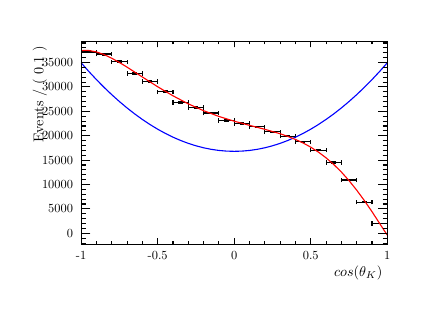
\begin{tikzpicture}
\pgfdeclareplotmark{cross} {
\pgfpathmoveto{\pgfpoint{-0.3\pgfplotmarksize}{\pgfplotmarksize}}
\pgfpathlineto{\pgfpoint{+0.3\pgfplotmarksize}{\pgfplotmarksize}}
\pgfpathlineto{\pgfpoint{+0.3\pgfplotmarksize}{0.3\pgfplotmarksize}}
\pgfpathlineto{\pgfpoint{+1\pgfplotmarksize}{0.3\pgfplotmarksize}}
\pgfpathlineto{\pgfpoint{+1\pgfplotmarksize}{-0.3\pgfplotmarksize}}
\pgfpathlineto{\pgfpoint{+0.3\pgfplotmarksize}{-0.3\pgfplotmarksize}}
\pgfpathlineto{\pgfpoint{+0.3\pgfplotmarksize}{-1.\pgfplotmarksize}}
\pgfpathlineto{\pgfpoint{-0.3\pgfplotmarksize}{-1.\pgfplotmarksize}}
\pgfpathlineto{\pgfpoint{-0.3\pgfplotmarksize}{-0.3\pgfplotmarksize}}
\pgfpathlineto{\pgfpoint{-1.\pgfplotmarksize}{-0.3\pgfplotmarksize}}
\pgfpathlineto{\pgfpoint{-1.\pgfplotmarksize}{0.3\pgfplotmarksize}}
\pgfpathlineto{\pgfpoint{-0.3\pgfplotmarksize}{0.3\pgfplotmarksize}}
\pgfpathclose
\pgfusepathqstroke
}
\pgfdeclareplotmark{cross*} {
\pgfpathmoveto{\pgfpoint{-0.3\pgfplotmarksize}{\pgfplotmarksize}}
\pgfpathlineto{\pgfpoint{+0.3\pgfplotmarksize}{\pgfplotmarksize}}
\pgfpathlineto{\pgfpoint{+0.3\pgfplotmarksize}{0.3\pgfplotmarksize}}
\pgfpathlineto{\pgfpoint{+1\pgfplotmarksize}{0.3\pgfplotmarksize}}
\pgfpathlineto{\pgfpoint{+1\pgfplotmarksize}{-0.3\pgfplotmarksize}}
\pgfpathlineto{\pgfpoint{+0.3\pgfplotmarksize}{-0.3\pgfplotmarksize}}
\pgfpathlineto{\pgfpoint{+0.3\pgfplotmarksize}{-1.\pgfplotmarksize}}
\pgfpathlineto{\pgfpoint{-0.3\pgfplotmarksize}{-1.\pgfplotmarksize}}
\pgfpathlineto{\pgfpoint{-0.3\pgfplotmarksize}{-0.3\pgfplotmarksize}}
\pgfpathlineto{\pgfpoint{-1.\pgfplotmarksize}{-0.3\pgfplotmarksize}}
\pgfpathlineto{\pgfpoint{-1.\pgfplotmarksize}{0.3\pgfplotmarksize}}
\pgfpathlineto{\pgfpoint{-0.3\pgfplotmarksize}{0.3\pgfplotmarksize}}
\pgfpathclose
\pgfusepathqfillstroke
}
\pgfdeclareplotmark{newstar} {
\pgfpathmoveto{\pgfqpoint{0pt}{\pgfplotmarksize}}
\pgfpathlineto{\pgfqpointpolar{44}{0.5\pgfplotmarksize}}
\pgfpathlineto{\pgfqpointpolar{18}{\pgfplotmarksize}}
\pgfpathlineto{\pgfqpointpolar{-20}{0.5\pgfplotmarksize}}
\pgfpathlineto{\pgfqpointpolar{-54}{\pgfplotmarksize}}
\pgfpathlineto{\pgfqpointpolar{-90}{0.5\pgfplotmarksize}}
\pgfpathlineto{\pgfqpointpolar{234}{\pgfplotmarksize}}
\pgfpathlineto{\pgfqpointpolar{198}{0.5\pgfplotmarksize}}
\pgfpathlineto{\pgfqpointpolar{162}{\pgfplotmarksize}}
\pgfpathlineto{\pgfqpointpolar{134}{0.5\pgfplotmarksize}}
\pgfpathclose
\pgfusepathqstroke
}
\pgfdeclareplotmark{newstar*} {
\pgfpathmoveto{\pgfqpoint{0pt}{\pgfplotmarksize}}
\pgfpathlineto{\pgfqpointpolar{44}{0.5\pgfplotmarksize}}
\pgfpathlineto{\pgfqpointpolar{18}{\pgfplotmarksize}}
\pgfpathlineto{\pgfqpointpolar{-20}{0.5\pgfplotmarksize}}
\pgfpathlineto{\pgfqpointpolar{-54}{\pgfplotmarksize}}
\pgfpathlineto{\pgfqpointpolar{-90}{0.5\pgfplotmarksize}}
\pgfpathlineto{\pgfqpointpolar{234}{\pgfplotmarksize}}
\pgfpathlineto{\pgfqpointpolar{198}{0.5\pgfplotmarksize}}
\pgfpathlineto{\pgfqpointpolar{162}{\pgfplotmarksize}}
\pgfpathlineto{\pgfqpointpolar{134}{0.5\pgfplotmarksize}}
\pgfpathclose
\pgfusepathqfillstroke
}
\definecolor{c}{rgb}{1,1,1};
\draw [color=c, fill=c] (0.1,3.47328) rectangle (4.9,6.74224);
\draw [color=c, fill=c] (0.772,3.99631) rectangle (4.66,6.57879);
\definecolor{c}{rgb}{0,0,0};
\draw [c] (0.772,3.99631) -- (0.772,6.57879) -- (4.66,6.57879) -- (4.66,3.99631) -- (0.772,3.99631);
\draw [c,line width=0.4] (0.772,3.99631) -- (4.66,3.99631);
\draw [anchor= east] (4.66,3.63855) node[scale=0.511737, rotate=0]{$cos(\theta_{K})$};
\draw [c,line width=0.4] (0.772,4.07575) -- (0.772,3.99631);
\draw [c,line width=0.4] (0.9664,4.03603) -- (0.9664,3.99631);
\draw [c,line width=0.4] (1.1608,4.03603) -- (1.1608,3.99631);
\draw [c,line width=0.4] (1.3552,4.03603) -- (1.3552,3.99631);
\draw [c,line width=0.4] (1.5496,4.03603) -- (1.5496,3.99631);
\draw [c,line width=0.4] (1.744,4.07575) -- (1.744,3.99631);
\draw [c,line width=0.4] (1.9384,4.03603) -- (1.9384,3.99631);
\draw [c,line width=0.4] (2.1328,4.03603) -- (2.1328,3.99631);
\draw [c,line width=0.4] (2.3272,4.03603) -- (2.3272,3.99631);
\draw [c,line width=0.4] (2.5216,4.03603) -- (2.5216,3.99631);
\draw [c,line width=0.4] (2.716,4.07575) -- (2.716,3.99631);
\draw [c,line width=0.4] (2.9104,4.03603) -- (2.9104,3.99631);
\draw [c,line width=0.4] (3.1048,4.03603) -- (3.1048,3.99631);
\draw [c,line width=0.4] (3.2992,4.03603) -- (3.2992,3.99631);
\draw [c,line width=0.4] (3.4936,4.03603) -- (3.4936,3.99631);
\draw [c,line width=0.4] (3.688,4.07575) -- (3.688,3.99631);
\draw [c,line width=0.4] (3.8824,4.03603) -- (3.8824,3.99631);
\draw [c,line width=0.4] (4.0768,4.03603) -- (4.0768,3.99631);
\draw [c,line width=0.4] (4.2712,4.03603) -- (4.2712,3.99631);
\draw [c,line width=0.4] (4.4656,4.03603) -- (4.4656,3.99631);
\draw [c,line width=0.4] (4.66,4.07575) -- (4.66,3.99631);
\draw [anchor=base] (0.772,3.80671) node[scale=0.44777, rotate=0]{-1};
\draw [anchor=base] (1.744,3.80671) node[scale=0.44777, rotate=0]{-0.5};
\draw [anchor=base] (2.716,3.80671) node[scale=0.44777, rotate=0]{0};
\draw [anchor=base] (3.688,3.80671) node[scale=0.44777, rotate=0]{0.5};
\draw [anchor=base] (4.66,3.80671) node[scale=0.44777, rotate=0]{1};
\draw [c,line width=0.4] (0.772,6.57879) -- (4.66,6.57879);
\draw [c,line width=0.4] (0.772,6.49936) -- (0.772,6.57879);
\draw [c,line width=0.4] (0.9664,6.53907) -- (0.9664,6.57879);
\draw [c,line width=0.4] (1.1608,6.53907) -- (1.1608,6.57879);
\draw [c,line width=0.4] (1.3552,6.53907) -- (1.3552,6.57879);
\draw [c,line width=0.4] (1.5496,6.53907) -- (1.5496,6.57879);
\draw [c,line width=0.4] (1.744,6.49936) -- (1.744,6.57879);
\draw [c,line width=0.4] (1.9384,6.53907) -- (1.9384,6.57879);
\draw [c,line width=0.4] (2.1328,6.53907) -- (2.1328,6.57879);
\draw [c,line width=0.4] (2.3272,6.53907) -- (2.3272,6.57879);
\draw [c,line width=0.4] (2.5216,6.53907) -- (2.5216,6.57879);
\draw [c,line width=0.4] (2.716,6.49936) -- (2.716,6.57879);
\draw [c,line width=0.4] (2.9104,6.53907) -- (2.9104,6.57879);
\draw [c,line width=0.4] (3.1048,6.53907) -- (3.1048,6.57879);
\draw [c,line width=0.4] (3.2992,6.53907) -- (3.2992,6.57879);
\draw [c,line width=0.4] (3.4936,6.53907) -- (3.4936,6.57879);
\draw [c,line width=0.4] (3.688,6.49936) -- (3.688,6.57879);
\draw [c,line width=0.4] (3.8824,6.53907) -- (3.8824,6.57879);
\draw [c,line width=0.4] (4.0768,6.53907) -- (4.0768,6.57879);
\draw [c,line width=0.4] (4.2712,6.53907) -- (4.2712,6.57879);
\draw [c,line width=0.4] (4.4656,6.53907) -- (4.4656,6.57879);
\draw [c,line width=0.4] (4.66,6.49936) -- (4.66,6.57879);
\draw [c,line width=0.4] (0.772,3.99631) -- (0.772,6.57879);
\draw [anchor= east] (0.246688,6.57879) node[scale=0.511737, rotate=90]{Events / ( 0.1 )};
\draw [c,line width=0.4] (0.88576,4.13775) -- (0.772,4.13775);
\draw [c,line width=0.4] (0.82888,4.19971) -- (0.772,4.19971);
\draw [c,line width=0.4] (0.82888,4.26167) -- (0.772,4.26167);
\draw [c,line width=0.4] (0.82888,4.32363) -- (0.772,4.32363);
\draw [c,line width=0.4] (0.82888,4.38559) -- (0.772,4.38559);
\draw [c,line width=0.4] (0.88576,4.44755) -- (0.772,4.44755);
\draw [c,line width=0.4] (0.82888,4.50951) -- (0.772,4.50951);
\draw [c,line width=0.4] (0.82888,4.57147) -- (0.772,4.57147);
\draw [c,line width=0.4] (0.82888,4.63343) -- (0.772,4.63343);
\draw [c,line width=0.4] (0.82888,4.69539) -- (0.772,4.69539);
\draw [c,line width=0.4] (0.88576,4.75735) -- (0.772,4.75735);
\draw [c,line width=0.4] (0.82888,4.81931) -- (0.772,4.81931);
\draw [c,line width=0.4] (0.82888,4.88128) -- (0.772,4.88128);
\draw [c,line width=0.4] (0.82888,4.94324) -- (0.772,4.94324);
\draw [c,line width=0.4] (0.82888,5.0052) -- (0.772,5.0052);
\draw [c,line width=0.4] (0.88576,5.06716) -- (0.772,5.06716);
\draw [c,line width=0.4] (0.82888,5.12912) -- (0.772,5.12912);
\draw [c,line width=0.4] (0.82888,5.19108) -- (0.772,5.19108);
\draw [c,line width=0.4] (0.82888,5.25304) -- (0.772,5.25304);
\draw [c,line width=0.4] (0.82888,5.315) -- (0.772,5.315);
\draw [c,line width=0.4] (0.88576,5.37696) -- (0.772,5.37696);
\draw [c,line width=0.4] (0.82888,5.43892) -- (0.772,5.43892);
\draw [c,line width=0.4] (0.82888,5.50088) -- (0.772,5.50088);
\draw [c,line width=0.4] (0.82888,5.56284) -- (0.772,5.56284);
\draw [c,line width=0.4] (0.82888,5.6248) -- (0.772,5.6248);
\draw [c,line width=0.4] (0.88576,5.68676) -- (0.772,5.68676);
\draw [c,line width=0.4] (0.82888,5.74872) -- (0.772,5.74872);
\draw [c,line width=0.4] (0.82888,5.81068) -- (0.772,5.81068);
\draw [c,line width=0.4] (0.82888,5.87264) -- (0.772,5.87264);
\draw [c,line width=0.4] (0.82888,5.9346) -- (0.772,5.9346);
\draw [c,line width=0.4] (0.88576,5.99656) -- (0.772,5.99656);
\draw [c,line width=0.4] (0.82888,6.05852) -- (0.772,6.05852);
\draw [c,line width=0.4] (0.82888,6.12048) -- (0.772,6.12048);
\draw [c,line width=0.4] (0.82888,6.18244) -- (0.772,6.18244);
\draw [c,line width=0.4] (0.82888,6.2444) -- (0.772,6.2444);
\draw [c,line width=0.4] (0.88576,6.30636) -- (0.772,6.30636);
\draw [c,line width=0.4] (0.88576,4.13775) -- (0.772,4.13775);
\draw [c,line width=0.4] (0.82888,4.07579) -- (0.772,4.07579);
\draw [c,line width=0.4] (0.82888,4.01383) -- (0.772,4.01383);
\draw [c,line width=0.4] (0.88576,6.30636) -- (0.772,6.30636);
\draw [c,line width=0.4] (0.82888,6.36832) -- (0.772,6.36832);
\draw [c,line width=0.4] (0.82888,6.43028) -- (0.772,6.43028);
\draw [c,line width=0.4] (0.82888,6.49225) -- (0.772,6.49225);
\draw [c,line width=0.4] (0.82888,6.55421) -- (0.772,6.55421);
\draw [anchor= east] (0.724,4.13775) node[scale=0.44777, rotate=0]{0};
\draw [anchor= east] (0.724,4.44755) node[scale=0.44777, rotate=0]{5000};
\draw [anchor= east] (0.724,4.75735) node[scale=0.44777, rotate=0]{10000};
\draw [anchor= east] (0.724,5.06716) node[scale=0.44777, rotate=0]{15000};
\draw [anchor= east] (0.724,5.37696) node[scale=0.44777, rotate=0]{20000};
\draw [anchor= east] (0.724,5.68676) node[scale=0.44777, rotate=0]{25000};
\draw [anchor= east] (0.724,5.99656) node[scale=0.44777, rotate=0]{30000};
\draw [anchor= east] (0.724,6.30636) node[scale=0.44777, rotate=0]{35000};
\draw [c,line width=0.4] (4.66,3.99631) -- (4.66,6.57879);
\draw [c,line width=0.4] (4.54624,4.13775) -- (4.66,4.13775);
\draw [c,line width=0.4] (4.60312,4.19971) -- (4.66,4.19971);
\draw [c,line width=0.4] (4.60312,4.26167) -- (4.66,4.26167);
\draw [c,line width=0.4] (4.60312,4.32363) -- (4.66,4.32363);
\draw [c,line width=0.4] (4.60312,4.38559) -- (4.66,4.38559);
\draw [c,line width=0.4] (4.54624,4.44755) -- (4.66,4.44755);
\draw [c,line width=0.4] (4.60312,4.50951) -- (4.66,4.50951);
\draw [c,line width=0.4] (4.60312,4.57147) -- (4.66,4.57147);
\draw [c,line width=0.4] (4.60312,4.63343) -- (4.66,4.63343);
\draw [c,line width=0.4] (4.60312,4.69539) -- (4.66,4.69539);
\draw [c,line width=0.4] (4.54624,4.75735) -- (4.66,4.75735);
\draw [c,line width=0.4] (4.60312,4.81931) -- (4.66,4.81931);
\draw [c,line width=0.4] (4.60312,4.88128) -- (4.66,4.88128);
\draw [c,line width=0.4] (4.60312,4.94324) -- (4.66,4.94324);
\draw [c,line width=0.4] (4.60312,5.0052) -- (4.66,5.0052);
\draw [c,line width=0.4] (4.54624,5.06716) -- (4.66,5.06716);
\draw [c,line width=0.4] (4.60312,5.12912) -- (4.66,5.12912);
\draw [c,line width=0.4] (4.60312,5.19108) -- (4.66,5.19108);
\draw [c,line width=0.4] (4.60312,5.25304) -- (4.66,5.25304);
\draw [c,line width=0.4] (4.60312,5.315) -- (4.66,5.315);
\draw [c,line width=0.4] (4.54624,5.37696) -- (4.66,5.37696);
\draw [c,line width=0.4] (4.60312,5.43892) -- (4.66,5.43892);
\draw [c,line width=0.4] (4.60312,5.50088) -- (4.66,5.50088);
\draw [c,line width=0.4] (4.60312,5.56284) -- (4.66,5.56284);
\draw [c,line width=0.4] (4.60312,5.6248) -- (4.66,5.6248);
\draw [c,line width=0.4] (4.54624,5.68676) -- (4.66,5.68676);
\draw [c,line width=0.4] (4.60312,5.74872) -- (4.66,5.74872);
\draw [c,line width=0.4] (4.60312,5.81068) -- (4.66,5.81068);
\draw [c,line width=0.4] (4.60312,5.87264) -- (4.66,5.87264);
\draw [c,line width=0.4] (4.60312,5.9346) -- (4.66,5.9346);
\draw [c,line width=0.4] (4.54624,5.99656) -- (4.66,5.99656);
\draw [c,line width=0.4] (4.60312,6.05852) -- (4.66,6.05852);
\draw [c,line width=0.4] (4.60312,6.12048) -- (4.66,6.12048);
\draw [c,line width=0.4] (4.60312,6.18244) -- (4.66,6.18244);
\draw [c,line width=0.4] (4.60312,6.2444) -- (4.66,6.2444);
\draw [c,line width=0.4] (4.54624,6.30636) -- (4.66,6.30636);
\draw [c,line width=0.4] (4.54624,4.13775) -- (4.66,4.13775);
\draw [c,line width=0.4] (4.60312,4.07579) -- (4.66,4.07579);
\draw [c,line width=0.4] (4.60312,4.01383) -- (4.66,4.01383);
\draw [c,line width=0.4] (4.54624,6.30636) -- (4.66,6.30636);
\draw [c,line width=0.4] (4.60312,6.36832) -- (4.66,6.36832);
\draw [c,line width=0.4] (4.60312,6.43028) -- (4.66,6.43028);
\draw [c,line width=0.4] (4.60312,6.49225) -- (4.66,6.49225);
\draw [c,line width=0.4] (4.60312,6.55421) -- (4.66,6.55421);
\draw [c,line width=0.4] (0.8692,6.44032) -- (0.772,6.44032);
\draw [c,line width=0.4] (0.772,6.41159) -- (0.772,6.46906);
\draw [c,line width=0.4] (0.8692,6.44032) -- (0.9664,6.44032);
\draw [c,line width=0.4] (0.9664,6.41159) -- (0.9664,6.46906);
\draw [c,line width=0.4] (0.8692,6.44032) -- (0.8692,6.4523);
\draw [c,line width=0.4] (0.840464,6.4523) -- (0.897936,6.4523);
\draw [c,line width=0.4] (0.8692,6.44032) -- (0.8692,6.42841);
\draw [c,line width=0.4] (0.840464,6.42841) -- (0.897936,6.42841);
\draw [c,line width=0.4] (1.0636,6.41455) -- (0.9664,6.41455);
\draw [c,line width=0.4] (0.9664,6.38581) -- (0.9664,6.44328);
\draw [c,line width=0.4] (1.0636,6.41455) -- (1.1608,6.41455);
\draw [c,line width=0.4] (1.1608,6.38581) -- (1.1608,6.44328);
\draw [c,line width=0.4] (1.0636,6.41455) -- (1.0636,6.42646);
\draw [c,line width=0.4] (1.03486,6.42646) -- (1.09234,6.42646);
\draw [c,line width=0.4] (1.0636,6.41455) -- (1.0636,6.4027);
\draw [c,line width=0.4] (1.03486,6.4027) -- (1.09234,6.4027);
\draw [c,line width=0.4] (1.258,6.3143) -- (1.1608,6.3143);
\draw [c,line width=0.4] (1.1608,6.28556) -- (1.1608,6.34303);
\draw [c,line width=0.4] (1.258,6.3143) -- (1.3552,6.3143);
\draw [c,line width=0.4] (1.3552,6.28556) -- (1.3552,6.34303);
\draw [c,line width=0.4] (1.258,6.3143) -- (1.258,6.32594);
\draw [c,line width=0.4] (1.22926,6.32594) -- (1.28674,6.32594);
\draw [c,line width=0.4] (1.258,6.3143) -- (1.258,6.30271);
\draw [c,line width=0.4] (1.22926,6.30271) -- (1.28674,6.30271);
\draw [c,line width=0.4] (1.4524,6.16999) -- (1.3552,6.16999);
\draw [c,line width=0.4] (1.3552,6.14125) -- (1.3552,6.19873);
\draw [c,line width=0.4] (1.4524,6.16999) -- (1.5496,6.16999);
\draw [c,line width=0.4] (1.5496,6.14125) -- (1.5496,6.19873);
\draw [c,line width=0.4] (1.4524,6.16999) -- (1.4524,6.18124);
\draw [c,line width=0.4] (1.42366,6.18124) -- (1.48114,6.18124);
\draw [c,line width=0.4] (1.4524,6.16999) -- (1.4524,6.1588);
\draw [c,line width=0.4] (1.42366,6.1588) -- (1.48114,6.1588);
\draw [c,line width=0.4] (1.6468,6.06286) -- (1.5496,6.06286);
\draw [c,line width=0.4] (1.5496,6.03412) -- (1.5496,6.0916);
\draw [c,line width=0.4] (1.6468,6.06286) -- (1.744,6.06286);
\draw [c,line width=0.4] (1.744,6.03412) -- (1.744,6.0916);
\draw [c,line width=0.4] (1.6468,6.06286) -- (1.6468,6.07381);
\draw [c,line width=0.4] (1.61806,6.07381) -- (1.67554,6.07381);
\draw [c,line width=0.4] (1.6468,6.06286) -- (1.6468,6.05197);
\draw [c,line width=0.4] (1.61806,6.05197) -- (1.67554,6.05197);
\draw [c,line width=0.4] (1.8412,5.93429) -- (1.744,5.93429);
\draw [c,line width=0.4] (1.744,5.90556) -- (1.744,5.96303);
\draw [c,line width=0.4] (1.8412,5.93429) -- (1.9384,5.93429);
\draw [c,line width=0.4] (1.9384,5.90556) -- (1.9384,5.96303);
\draw [c,line width=0.4] (1.8412,5.93429) -- (1.8412,5.94487);
\draw [c,line width=0.4] (1.81246,5.94487) -- (1.86994,5.94487);
\draw [c,line width=0.4] (1.8412,5.93429) -- (1.8412,5.92377);
\draw [c,line width=0.4] (1.81246,5.92377) -- (1.86994,5.92377);
\draw [c,line width=0.4] (2.0356,5.80188) -- (1.9384,5.80188);
\draw [c,line width=0.4] (1.9384,5.77315) -- (1.9384,5.83062);
\draw [c,line width=0.4] (2.0356,5.80188) -- (2.1328,5.80188);
\draw [c,line width=0.4] (2.1328,5.77315) -- (2.1328,5.83062);
\draw [c,line width=0.4] (2.0356,5.80188) -- (2.0356,5.81207);
\draw [c,line width=0.4] (2.00686,5.81207) -- (2.06434,5.81207);
\draw [c,line width=0.4] (2.0356,5.80188) -- (2.0356,5.79176);
\draw [c,line width=0.4] (2.00686,5.79176) -- (2.06434,5.79176);
\draw [c,line width=0.4] (2.23,5.73813) -- (2.1328,5.73813);
\draw [c,line width=0.4] (2.1328,5.70939) -- (2.1328,5.76686);
\draw [c,line width=0.4] (2.23,5.73813) -- (2.3272,5.73813);
\draw [c,line width=0.4] (2.3272,5.70939) -- (2.3272,5.76686);
\draw [c,line width=0.4] (2.23,5.73813) -- (2.23,5.74811);
\draw [c,line width=0.4] (2.20126,5.74811) -- (2.25874,5.74811);
\draw [c,line width=0.4] (2.23,5.73813) -- (2.23,5.7282);
\draw [c,line width=0.4] (2.20126,5.7282) -- (2.25874,5.7282);
\draw [c,line width=0.4] (2.4244,5.66545) -- (2.3272,5.66545);
\draw [c,line width=0.4] (2.3272,5.63671) -- (2.3272,5.69418);
\draw [c,line width=0.4] (2.4244,5.66545) -- (2.5216,5.66545);
\draw [c,line width=0.4] (2.5216,5.63671) -- (2.5216,5.69418);
\draw [c,line width=0.4] (2.4244,5.66545) -- (2.4244,5.67521);
\draw [c,line width=0.4] (2.39566,5.67521) -- (2.45314,5.67521);
\draw [c,line width=0.4] (2.4244,5.66545) -- (2.4244,5.65575);
\draw [c,line width=0.4] (2.39566,5.65575) -- (2.45314,5.65575);
\draw [c,line width=0.4] (2.6188,5.57003) -- (2.5216,5.57003);
\draw [c,line width=0.4] (2.5216,5.54129) -- (2.5216,5.59876);
\draw [c,line width=0.4] (2.6188,5.57003) -- (2.716,5.57003);
\draw [c,line width=0.4] (2.716,5.54129) -- (2.716,5.59876);
\draw [c,line width=0.4] (2.6188,5.57003) -- (2.6188,5.57948);
\draw [c,line width=0.4] (2.59006,5.57948) -- (2.64754,5.57948);
\draw [c,line width=0.4] (2.6188,5.57003) -- (2.6188,5.56064);
\draw [c,line width=0.4] (2.59006,5.56064) -- (2.64754,5.56064);
\draw [c,line width=0.4] (2.8132,5.53068) -- (2.716,5.53068);
\draw [c,line width=0.4] (2.716,5.50195) -- (2.716,5.55942);
\draw [c,line width=0.4] (2.8132,5.53068) -- (2.9104,5.53068);
\draw [c,line width=0.4] (2.9104,5.50195) -- (2.9104,5.55942);
\draw [c,line width=0.4] (2.8132,5.53068) -- (2.8132,5.54);
\draw [c,line width=0.4] (2.78446,5.54) -- (2.84194,5.54);
\draw [c,line width=0.4] (2.8132,5.53068) -- (2.8132,5.52142);
\draw [c,line width=0.4] (2.78446,5.52142) -- (2.84194,5.52142);
\draw [c,line width=0.4] (3.0076,5.48874) -- (2.9104,5.48874);
\draw [c,line width=0.4] (2.9104,5.46) -- (2.9104,5.51747);
\draw [c,line width=0.4] (3.0076,5.48874) -- (3.1048,5.48874);
\draw [c,line width=0.4] (3.1048,5.46) -- (3.1048,5.51747);
\draw [c,line width=0.4] (3.0076,5.48874) -- (3.0076,5.49792);
\draw [c,line width=0.4] (2.97886,5.49792) -- (3.03634,5.49792);
\draw [c,line width=0.4] (3.0076,5.48874) -- (3.0076,5.47962);
\draw [c,line width=0.4] (2.97886,5.47962) -- (3.03634,5.47962);
\draw [c,line width=0.4] (3.202,5.42647) -- (3.1048,5.42647);
\draw [c,line width=0.4] (3.1048,5.39773) -- (3.1048,5.4552);
\draw [c,line width=0.4] (3.202,5.42647) -- (3.2992,5.42647);
\draw [c,line width=0.4] (3.2992,5.39773) -- (3.2992,5.4552);
\draw [c,line width=0.4] (3.202,5.42647) -- (3.202,5.43543);
\draw [c,line width=0.4] (3.17326,5.43543) -- (3.23074,5.43543);
\draw [c,line width=0.4] (3.202,5.42647) -- (3.202,5.41756);
\draw [c,line width=0.4] (3.17326,5.41756) -- (3.23074,5.41756);
\draw [c,line width=0.4] (3.3964,5.37107) -- (3.2992,5.37107);
\draw [c,line width=0.4] (3.2992,5.34234) -- (3.2992,5.39981);
\draw [c,line width=0.4] (3.3964,5.37107) -- (3.4936,5.37107);
\draw [c,line width=0.4] (3.4936,5.34234) -- (3.4936,5.39981);
\draw [c,line width=0.4] (3.3964,5.37107) -- (3.3964,5.37985);
\draw [c,line width=0.4] (3.36766,5.37985) -- (3.42514,5.37985);
\draw [c,line width=0.4] (3.3964,5.37107) -- (3.3964,5.36236);
\draw [c,line width=0.4] (3.36766,5.36236) -- (3.42514,5.36236);
\draw [c,line width=0.4] (3.5908,5.29883) -- (3.4936,5.29883);
\draw [c,line width=0.4] (3.4936,5.27009) -- (3.4936,5.32756);
\draw [c,line width=0.4] (3.5908,5.29883) -- (3.688,5.29883);
\draw [c,line width=0.4] (3.688,5.27009) -- (3.688,5.32756);
\draw [c,line width=0.4] (3.5908,5.29883) -- (3.5908,5.30734);
\draw [c,line width=0.4] (3.56206,5.30734) -- (3.61954,5.30734);
\draw [c,line width=0.4] (3.5908,5.29883) -- (3.5908,5.29038);
\draw [c,line width=0.4] (3.56206,5.29038) -- (3.61954,5.29038);
\draw [c,line width=0.4] (3.7852,5.19442) -- (3.688,5.19442);
\draw [c,line width=0.4] (3.688,5.16569) -- (3.688,5.22316);
\draw [c,line width=0.4] (3.7852,5.19442) -- (3.8824,5.19442);
\draw [c,line width=0.4] (3.8824,5.16569) -- (3.8824,5.22316);
\draw [c,line width=0.4] (3.7852,5.19442) -- (3.7852,5.20255);
\draw [c,line width=0.4] (3.75646,5.20255) -- (3.81394,5.20255);
\draw [c,line width=0.4] (3.7852,5.19442) -- (3.7852,5.18636);
\draw [c,line width=0.4] (3.75646,5.18636) -- (3.81394,5.18636);
\draw [c,line width=0.4] (3.9796,5.03642) -- (3.8824,5.03642);
\draw [c,line width=0.4] (3.8824,5.00769) -- (3.8824,5.06516);
\draw [c,line width=0.4] (3.9796,5.03642) -- (4.0768,5.03642);
\draw [c,line width=0.4] (4.0768,5.00769) -- (4.0768,5.06516);
\draw [c,line width=0.4] (3.9796,5.03642) -- (3.9796,5.04392);
\draw [c,line width=0.4] (3.95086,5.04392) -- (4.00834,5.04392);
\draw [c,line width=0.4] (3.9796,5.03642) -- (3.9796,5.02899);
\draw [c,line width=0.4] (3.95086,5.02899) -- (4.00834,5.02899);
\draw [c,line width=0.4] (4.174,4.8151) -- (4.0768,4.8151);
\draw [c,line width=0.4] (4.0768,4.78637) -- (4.0768,4.84384);
\draw [c,line width=0.4] (4.174,4.8151) -- (4.2712,4.8151);
\draw [c,line width=0.4] (4.2712,4.78637) -- (4.2712,4.84384);
\draw [c,line width=0.4] (4.174,4.8151) -- (4.174,4.82161);
\draw [c,line width=0.4] (4.14526,4.82161) -- (4.20274,4.82161);
\draw [c,line width=0.4] (4.174,4.8151) -- (4.174,4.80865);
\draw [c,line width=0.4] (4.14526,4.80865) -- (4.20274,4.80865);
\draw [c,line width=0.4] (4.3684,4.53343) -- (4.2712,4.53343);
\draw [c,line width=0.4] (4.2712,4.50469) -- (4.2712,4.56217);
\draw [c,line width=0.4] (4.3684,4.53343) -- (4.4656,4.53343);
\draw [c,line width=0.4] (4.4656,4.50469) -- (4.4656,4.56217);
\draw [c,line width=0.4] (4.3684,4.53343) -- (4.3684,4.53841);
\draw [c,line width=0.4] (4.33966,4.53841) -- (4.39714,4.53841);
\draw [c,line width=0.4] (4.3684,4.53343) -- (4.3684,4.52851);
\draw [c,line width=0.4] (4.33966,4.52851) -- (4.39714,4.52851);
\draw [c,line width=0.4] (4.5628,4.26322) -- (4.4656,4.26322);
\draw [c,line width=0.4] (4.4656,4.23448) -- (4.4656,4.29196);
\draw [c,line width=0.4] (4.5628,4.26322) -- (4.66,4.26322);
\draw [c,line width=0.4] (4.66,4.23448) -- (4.66,4.29196);
\draw [c,line width=0.4] (4.5628,4.26322) -- (4.5628,4.26604);
\draw [c,line width=0.4] (4.53406,4.26604) -- (4.59154,4.26604);
\draw [c,line width=0.4] (4.5628,4.26322) -- (4.5628,4.26046);
\draw [c,line width=0.4] (4.53406,4.26046) -- (4.59154,4.26046);
\foreach \P in
 {(0.8692,6.44032),(1.0636,6.41455),(1.258,6.3143),(1.4524,6.16999),(1.6468,6.06286),(1.8412,5.93429),(2.0356,5.80188),(2.23,5.73813),(2.4244,5.66545),(2.6188,5.57003),(2.8132,5.53068),(3.0076,5.48874),(3.202,5.42647),(3.3964,5.37107),(3.5908,5.29883
),(3.7852,5.19442),(3.9796,5.03642),(4.174,4.8151),(4.3684,4.53343),(4.5628,4.26322)}{\draw[mark options={color=c,fill=c},mark size=0.960961pt,mark=] plot coordinates {\P};}
\definecolor{c}{rgb}{0,0,1};
\draw [c,line width=0.4] (0.772,6.30299) -- (0.772,6.30299);
\draw [c,line width=0.4] (0.772,6.30299) -- (0.8692,6.19338) -- (0.9664,6.08939) -- (1.0636,5.99102) -- (1.1608,5.89827) -- (1.258,5.81114) -- (1.3552,5.72964) -- (1.4524,5.65375) -- (1.5496,5.58349) -- (1.6468,5.51884) -- (1.744,5.45982) --
 (1.8412,5.40642) -- (1.9384,5.35864) -- (2.0356,5.31648) -- (2.1328,5.27995) -- (2.23,5.24903) -- (2.3272,5.22373) -- (2.4244,5.20406) -- (2.5216,5.19001) -- (2.6188,5.18158) -- (2.716,5.17877) -- (2.8132,5.18158) -- (2.9104,5.19001) --
 (3.0076,5.20406) -- (3.1048,5.22373) -- (3.202,5.24903) -- (3.2992,5.27995) -- (3.3964,5.31648) -- (3.4936,5.35864) -- (3.5908,5.40642) -- (3.688,5.45982) -- (3.7852,5.51884) -- (3.8824,5.58349) -- (3.9796,5.65375) -- (4.0768,5.72964) --
 (4.174,5.81114) -- (4.2712,5.89827) -- (4.3684,5.99102) -- (4.4656,6.08939) -- (4.5628,6.19338) -- (4.66,6.30299) -- (4.66,6.30299) -- (4.66,6.30299);
\definecolor{c}{rgb}{1,0,0};
\draw [c,line width=0.4] (0.772,6.45693) -- (0.772,6.45693);
\draw [c,line width=0.4] (0.772,6.45693) -- (0.8206,6.46141) -- (0.8692,6.4598) -- (0.9664,6.44136) -- (1.0636,6.40695) -- (1.1608,6.36098) -- (1.258,6.30698) -- (1.3552,6.24784) -- (1.5496,6.12277) -- (1.744,5.99883) -- (1.9384,5.8838) --
 (2.1328,5.78187) -- (2.3272,5.6947) -- (2.5216,5.62192) -- (2.716,5.56133) -- (2.9104,5.50883) -- (3.1048,5.45838) -- (3.2992,5.40199) -- (3.3964,5.36859) -- (3.4936,5.32996) -- (3.5908,5.28476) -- (3.688,5.2316) -- (3.7852,5.16919) --
 (3.8824,5.09635) -- (3.9796,5.0121) -- (4.0768,4.91576) -- (4.174,4.80705) -- (4.2712,4.68622) -- (4.3684,4.55419) -- (4.4656,4.41271) -- (4.66,4.1137) -- (4.66,4.1137) -- (4.66,4.1137);
\definecolor{c}{rgb}{0,0,0};
\draw [c,line width=0.4] (0.772,3.99631) -- (4.66,3.99631);
\draw [c,line width=0.4] (0.772,4.07575) -- (0.772,3.99631);
\draw [c,line width=0.4] (0.9664,4.03603) -- (0.9664,3.99631);
\draw [c,line width=0.4] (1.1608,4.03603) -- (1.1608,3.99631);
\draw [c,line width=0.4] (1.3552,4.03603) -- (1.3552,3.99631);
\draw [c,line width=0.4] (1.5496,4.03603) -- (1.5496,3.99631);
\draw [c,line width=0.4] (1.744,4.07575) -- (1.744,3.99631);
\draw [c,line width=0.4] (1.9384,4.03603) -- (1.9384,3.99631);
\draw [c,line width=0.4] (2.1328,4.03603) -- (2.1328,3.99631);
\draw [c,line width=0.4] (2.3272,4.03603) -- (2.3272,3.99631);
\draw [c,line width=0.4] (2.5216,4.03603) -- (2.5216,3.99631);
\draw [c,line width=0.4] (2.716,4.07575) -- (2.716,3.99631);
\draw [c,line width=0.4] (2.9104,4.03603) -- (2.9104,3.99631);
\draw [c,line width=0.4] (3.1048,4.03603) -- (3.1048,3.99631);
\draw [c,line width=0.4] (3.2992,4.03603) -- (3.2992,3.99631);
\draw [c,line width=0.4] (3.4936,4.03603) -- (3.4936,3.99631);
\draw [c,line width=0.4] (3.688,4.07575) -- (3.688,3.99631);
\draw [c,line width=0.4] (3.8824,4.03603) -- (3.8824,3.99631);
\draw [c,line width=0.4] (4.0768,4.03603) -- (4.0768,3.99631);
\draw [c,line width=0.4] (4.2712,4.03603) -- (4.2712,3.99631);
\draw [c,line width=0.4] (4.4656,4.03603) -- (4.4656,3.99631);
\draw [c,line width=0.4] (4.66,4.07575) -- (4.66,3.99631);
\draw [c,line width=0.4] (0.772,6.57879) -- (4.66,6.57879);
\draw [c,line width=0.4] (0.772,6.49936) -- (0.772,6.57879);
\draw [c,line width=0.4] (0.9664,6.53907) -- (0.9664,6.57879);
\draw [c,line width=0.4] (1.1608,6.53907) -- (1.1608,6.57879);
\draw [c,line width=0.4] (1.3552,6.53907) -- (1.3552,6.57879);
\draw [c,line width=0.4] (1.5496,6.53907) -- (1.5496,6.57879);
\draw [c,line width=0.4] (1.744,6.49936) -- (1.744,6.57879);
\draw [c,line width=0.4] (1.9384,6.53907) -- (1.9384,6.57879);
\draw [c,line width=0.4] (2.1328,6.53907) -- (2.1328,6.57879);
\draw [c,line width=0.4] (2.3272,6.53907) -- (2.3272,6.57879);
\draw [c,line width=0.4] (2.5216,6.53907) -- (2.5216,6.57879);
\draw [c,line width=0.4] (2.716,6.49936) -- (2.716,6.57879);
\draw [c,line width=0.4] (2.9104,6.53907) -- (2.9104,6.57879);
\draw [c,line width=0.4] (3.1048,6.53907) -- (3.1048,6.57879);
\draw [c,line width=0.4] (3.2992,6.53907) -- (3.2992,6.57879);
\draw [c,line width=0.4] (3.4936,6.53907) -- (3.4936,6.57879);
\draw [c,line width=0.4] (3.688,6.49936) -- (3.688,6.57879);
\draw [c,line width=0.4] (3.8824,6.53907) -- (3.8824,6.57879);
\draw [c,line width=0.4] (4.0768,6.53907) -- (4.0768,6.57879);
\draw [c,line width=0.4] (4.2712,6.53907) -- (4.2712,6.57879);
\draw [c,line width=0.4] (4.4656,6.53907) -- (4.4656,6.57879);
\draw [c,line width=0.4] (4.66,6.49936) -- (4.66,6.57879);
\draw [c,line width=0.4] (0.772,3.99631) -- (0.772,6.57879);
\draw [c,line width=0.4] (0.88576,4.13775) -- (0.772,4.13775);
\draw [c,line width=0.4] (0.82888,4.19971) -- (0.772,4.19971);
\draw [c,line width=0.4] (0.82888,4.26167) -- (0.772,4.26167);
\draw [c,line width=0.4] (0.82888,4.32363) -- (0.772,4.32363);
\draw [c,line width=0.4] (0.82888,4.38559) -- (0.772,4.38559);
\draw [c,line width=0.4] (0.88576,4.44755) -- (0.772,4.44755);
\draw [c,line width=0.4] (0.82888,4.50951) -- (0.772,4.50951);
\draw [c,line width=0.4] (0.82888,4.57147) -- (0.772,4.57147);
\draw [c,line width=0.4] (0.82888,4.63343) -- (0.772,4.63343);
\draw [c,line width=0.4] (0.82888,4.69539) -- (0.772,4.69539);
\draw [c,line width=0.4] (0.88576,4.75735) -- (0.772,4.75735);
\draw [c,line width=0.4] (0.82888,4.81931) -- (0.772,4.81931);
\draw [c,line width=0.4] (0.82888,4.88128) -- (0.772,4.88128);
\draw [c,line width=0.4] (0.82888,4.94324) -- (0.772,4.94324);
\draw [c,line width=0.4] (0.82888,5.0052) -- (0.772,5.0052);
\draw [c,line width=0.4] (0.88576,5.06716) -- (0.772,5.06716);
\draw [c,line width=0.4] (0.82888,5.12912) -- (0.772,5.12912);
\draw [c,line width=0.4] (0.82888,5.19108) -- (0.772,5.19108);
\draw [c,line width=0.4] (0.82888,5.25304) -- (0.772,5.25304);
\draw [c,line width=0.4] (0.82888,5.315) -- (0.772,5.315);
\draw [c,line width=0.4] (0.88576,5.37696) -- (0.772,5.37696);
\draw [c,line width=0.4] (0.82888,5.43892) -- (0.772,5.43892);
\draw [c,line width=0.4] (0.82888,5.50088) -- (0.772,5.50088);
\draw [c,line width=0.4] (0.82888,5.56284) -- (0.772,5.56284);
\draw [c,line width=0.4] (0.82888,5.6248) -- (0.772,5.6248);
\draw [c,line width=0.4] (0.88576,5.68676) -- (0.772,5.68676);
\draw [c,line width=0.4] (0.82888,5.74872) -- (0.772,5.74872);
\draw [c,line width=0.4] (0.82888,5.81068) -- (0.772,5.81068);
\draw [c,line width=0.4] (0.82888,5.87264) -- (0.772,5.87264);
\draw [c,line width=0.4] (0.82888,5.9346) -- (0.772,5.9346);
\draw [c,line width=0.4] (0.88576,5.99656) -- (0.772,5.99656);
\draw [c,line width=0.4] (0.82888,6.05852) -- (0.772,6.05852);
\draw [c,line width=0.4] (0.82888,6.12048) -- (0.772,6.12048);
\draw [c,line width=0.4] (0.82888,6.18244) -- (0.772,6.18244);
\draw [c,line width=0.4] (0.82888,6.2444) -- (0.772,6.2444);
\draw [c,line width=0.4] (0.88576,6.30636) -- (0.772,6.30636);
\draw [c,line width=0.4] (0.88576,4.13775) -- (0.772,4.13775);
\draw [c,line width=0.4] (0.82888,4.07579) -- (0.772,4.07579);
\draw [c,line width=0.4] (0.82888,4.01383) -- (0.772,4.01383);
\draw [c,line width=0.4] (0.88576,6.30636) -- (0.772,6.30636);
\draw [c,line width=0.4] (0.82888,6.36832) -- (0.772,6.36832);
\draw [c,line width=0.4] (0.82888,6.43028) -- (0.772,6.43028);
\draw [c,line width=0.4] (0.82888,6.49225) -- (0.772,6.49225);
\draw [c,line width=0.4] (0.82888,6.55421) -- (0.772,6.55421);
\draw [c,line width=0.4] (4.66,3.99631) -- (4.66,6.57879);
\draw [c,line width=0.4] (4.54624,4.13775) -- (4.66,4.13775);
\draw [c,line width=0.4] (4.60312,4.19971) -- (4.66,4.19971);
\draw [c,line width=0.4] (4.60312,4.26167) -- (4.66,4.26167);
\draw [c,line width=0.4] (4.60312,4.32363) -- (4.66,4.32363);
\draw [c,line width=0.4] (4.60312,4.38559) -- (4.66,4.38559);
\draw [c,line width=0.4] (4.54624,4.44755) -- (4.66,4.44755);
\draw [c,line width=0.4] (4.60312,4.50951) -- (4.66,4.50951);
\draw [c,line width=0.4] (4.60312,4.57147) -- (4.66,4.57147);
\draw [c,line width=0.4] (4.60312,4.63343) -- (4.66,4.63343);
\draw [c,line width=0.4] (4.60312,4.69539) -- (4.66,4.69539);
\draw [c,line width=0.4] (4.54624,4.75735) -- (4.66,4.75735);
\draw [c,line width=0.4] (4.60312,4.81931) -- (4.66,4.81931);
\draw [c,line width=0.4] (4.60312,4.88128) -- (4.66,4.88128);
\draw [c,line width=0.4] (4.60312,4.94324) -- (4.66,4.94324);
\draw [c,line width=0.4] (4.60312,5.0052) -- (4.66,5.0052);
\draw [c,line width=0.4] (4.54624,5.06716) -- (4.66,5.06716);
\draw [c,line width=0.4] (4.60312,5.12912) -- (4.66,5.12912);
\draw [c,line width=0.4] (4.60312,5.19108) -- (4.66,5.19108);
\draw [c,line width=0.4] (4.60312,5.25304) -- (4.66,5.25304);
\draw [c,line width=0.4] (4.60312,5.315) -- (4.66,5.315);
\draw [c,line width=0.4] (4.54624,5.37696) -- (4.66,5.37696);
\draw [c,line width=0.4] (4.60312,5.43892) -- (4.66,5.43892);
\draw [c,line width=0.4] (4.60312,5.50088) -- (4.66,5.50088);
\draw [c,line width=0.4] (4.60312,5.56284) -- (4.66,5.56284);
\draw [c,line width=0.4] (4.60312,5.6248) -- (4.66,5.6248);
\draw [c,line width=0.4] (4.54624,5.68676) -- (4.66,5.68676);
\draw [c,line width=0.4] (4.60312,5.74872) -- (4.66,5.74872);
\draw [c,line width=0.4] (4.60312,5.81068) -- (4.66,5.81068);
\draw [c,line width=0.4] (4.60312,5.87264) -- (4.66,5.87264);
\draw [c,line width=0.4] (4.60312,5.9346) -- (4.66,5.9346);
\draw [c,line width=0.4] (4.54624,5.99656) -- (4.66,5.99656);
\draw [c,line width=0.4] (4.60312,6.05852) -- (4.66,6.05852);
\draw [c,line width=0.4] (4.60312,6.12048) -- (4.66,6.12048);
\draw [c,line width=0.4] (4.60312,6.18244) -- (4.66,6.18244);
\draw [c,line width=0.4] (4.60312,6.2444) -- (4.66,6.2444);
\draw [c,line width=0.4] (4.54624,6.30636) -- (4.66,6.30636);
\draw [c,line width=0.4] (4.54624,4.13775) -- (4.66,4.13775);
\draw [c,line width=0.4] (4.60312,4.07579) -- (4.66,4.07579);
\draw [c,line width=0.4] (4.60312,4.01383) -- (4.66,4.01383);
\draw [c,line width=0.4] (4.54624,6.30636) -- (4.66,6.30636);
\draw [c,line width=0.4] (4.60312,6.36832) -- (4.66,6.36832);
\draw [c,line width=0.4] (4.60312,6.43028) -- (4.66,6.43028);
\draw [c,line width=0.4] (4.60312,6.49225) -- (4.66,6.49225);
\draw [c,line width=0.4] (4.60312,6.55421) -- (4.66,6.55421);
\end{tikzpicture}
}
    \caption{}
    \label{angAcc_nom}
  \end{subfigure}%
  \hfill%
  \begin{subfigure}{0.5\textwidth}
    \scalebox{1.3}{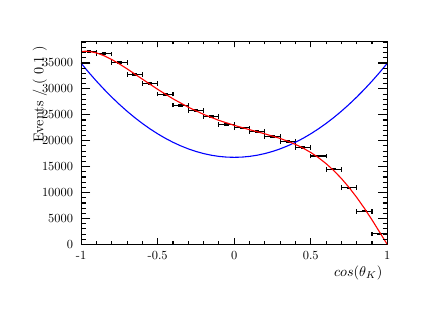
\begin{tikzpicture}
\pgfdeclareplotmark{cross} {
\pgfpathmoveto{\pgfpoint{-0.3\pgfplotmarksize}{\pgfplotmarksize}}
\pgfpathlineto{\pgfpoint{+0.3\pgfplotmarksize}{\pgfplotmarksize}}
\pgfpathlineto{\pgfpoint{+0.3\pgfplotmarksize}{0.3\pgfplotmarksize}}
\pgfpathlineto{\pgfpoint{+1\pgfplotmarksize}{0.3\pgfplotmarksize}}
\pgfpathlineto{\pgfpoint{+1\pgfplotmarksize}{-0.3\pgfplotmarksize}}
\pgfpathlineto{\pgfpoint{+0.3\pgfplotmarksize}{-0.3\pgfplotmarksize}}
\pgfpathlineto{\pgfpoint{+0.3\pgfplotmarksize}{-1.\pgfplotmarksize}}
\pgfpathlineto{\pgfpoint{-0.3\pgfplotmarksize}{-1.\pgfplotmarksize}}
\pgfpathlineto{\pgfpoint{-0.3\pgfplotmarksize}{-0.3\pgfplotmarksize}}
\pgfpathlineto{\pgfpoint{-1.\pgfplotmarksize}{-0.3\pgfplotmarksize}}
\pgfpathlineto{\pgfpoint{-1.\pgfplotmarksize}{0.3\pgfplotmarksize}}
\pgfpathlineto{\pgfpoint{-0.3\pgfplotmarksize}{0.3\pgfplotmarksize}}
\pgfpathclose
\pgfusepathqstroke
}
\pgfdeclareplotmark{cross*} {
\pgfpathmoveto{\pgfpoint{-0.3\pgfplotmarksize}{\pgfplotmarksize}}
\pgfpathlineto{\pgfpoint{+0.3\pgfplotmarksize}{\pgfplotmarksize}}
\pgfpathlineto{\pgfpoint{+0.3\pgfplotmarksize}{0.3\pgfplotmarksize}}
\pgfpathlineto{\pgfpoint{+1\pgfplotmarksize}{0.3\pgfplotmarksize}}
\pgfpathlineto{\pgfpoint{+1\pgfplotmarksize}{-0.3\pgfplotmarksize}}
\pgfpathlineto{\pgfpoint{+0.3\pgfplotmarksize}{-0.3\pgfplotmarksize}}
\pgfpathlineto{\pgfpoint{+0.3\pgfplotmarksize}{-1.\pgfplotmarksize}}
\pgfpathlineto{\pgfpoint{-0.3\pgfplotmarksize}{-1.\pgfplotmarksize}}
\pgfpathlineto{\pgfpoint{-0.3\pgfplotmarksize}{-0.3\pgfplotmarksize}}
\pgfpathlineto{\pgfpoint{-1.\pgfplotmarksize}{-0.3\pgfplotmarksize}}
\pgfpathlineto{\pgfpoint{-1.\pgfplotmarksize}{0.3\pgfplotmarksize}}
\pgfpathlineto{\pgfpoint{-0.3\pgfplotmarksize}{0.3\pgfplotmarksize}}
\pgfpathclose
\pgfusepathqfillstroke
}
\pgfdeclareplotmark{newstar} {
\pgfpathmoveto{\pgfqpoint{0pt}{\pgfplotmarksize}}
\pgfpathlineto{\pgfqpointpolar{44}{0.5\pgfplotmarksize}}
\pgfpathlineto{\pgfqpointpolar{18}{\pgfplotmarksize}}
\pgfpathlineto{\pgfqpointpolar{-20}{0.5\pgfplotmarksize}}
\pgfpathlineto{\pgfqpointpolar{-54}{\pgfplotmarksize}}
\pgfpathlineto{\pgfqpointpolar{-90}{0.5\pgfplotmarksize}}
\pgfpathlineto{\pgfqpointpolar{234}{\pgfplotmarksize}}
\pgfpathlineto{\pgfqpointpolar{198}{0.5\pgfplotmarksize}}
\pgfpathlineto{\pgfqpointpolar{162}{\pgfplotmarksize}}
\pgfpathlineto{\pgfqpointpolar{134}{0.5\pgfplotmarksize}}
\pgfpathclose
\pgfusepathqstroke
}
\pgfdeclareplotmark{newstar*} {
\pgfpathmoveto{\pgfqpoint{0pt}{\pgfplotmarksize}}
\pgfpathlineto{\pgfqpointpolar{44}{0.5\pgfplotmarksize}}
\pgfpathlineto{\pgfqpointpolar{18}{\pgfplotmarksize}}
\pgfpathlineto{\pgfqpointpolar{-20}{0.5\pgfplotmarksize}}
\pgfpathlineto{\pgfqpointpolar{-54}{\pgfplotmarksize}}
\pgfpathlineto{\pgfqpointpolar{-90}{0.5\pgfplotmarksize}}
\pgfpathlineto{\pgfqpointpolar{234}{\pgfplotmarksize}}
\pgfpathlineto{\pgfqpointpolar{198}{0.5\pgfplotmarksize}}
\pgfpathlineto{\pgfqpointpolar{162}{\pgfplotmarksize}}
\pgfpathlineto{\pgfqpointpolar{134}{0.5\pgfplotmarksize}}
\pgfpathclose
\pgfusepathqfillstroke
}
\definecolor{c}{rgb}{1,1,1};
\draw [color=c, fill=c] (0.1,3.47328) rectangle (4.9,6.74224);
\draw [color=c, fill=c] (0.772,3.99631) rectangle (4.66,6.57879);
\definecolor{c}{rgb}{0,0,0};
\draw [c] (0.772,3.99631) -- (0.772,6.57879) -- (4.66,6.57879) -- (4.66,3.99631) -- (0.772,3.99631);
\draw [c,line width=0.4] (0.772,3.99631) -- (4.66,3.99631);
\draw [anchor= east] (4.66,3.63855) node[scale=0.511737, rotate=0]{$cos(\theta_{K})$};
\draw [c,line width=0.4] (0.772,4.07575) -- (0.772,3.99631);
\draw [c,line width=0.4] (0.9664,4.03603) -- (0.9664,3.99631);
\draw [c,line width=0.4] (1.1608,4.03603) -- (1.1608,3.99631);
\draw [c,line width=0.4] (1.3552,4.03603) -- (1.3552,3.99631);
\draw [c,line width=0.4] (1.5496,4.03603) -- (1.5496,3.99631);
\draw [c,line width=0.4] (1.744,4.07575) -- (1.744,3.99631);
\draw [c,line width=0.4] (1.9384,4.03603) -- (1.9384,3.99631);
\draw [c,line width=0.4] (2.1328,4.03603) -- (2.1328,3.99631);
\draw [c,line width=0.4] (2.3272,4.03603) -- (2.3272,3.99631);
\draw [c,line width=0.4] (2.5216,4.03603) -- (2.5216,3.99631);
\draw [c,line width=0.4] (2.716,4.07575) -- (2.716,3.99631);
\draw [c,line width=0.4] (2.9104,4.03603) -- (2.9104,3.99631);
\draw [c,line width=0.4] (3.1048,4.03603) -- (3.1048,3.99631);
\draw [c,line width=0.4] (3.2992,4.03603) -- (3.2992,3.99631);
\draw [c,line width=0.4] (3.4936,4.03603) -- (3.4936,3.99631);
\draw [c,line width=0.4] (3.688,4.07575) -- (3.688,3.99631);
\draw [c,line width=0.4] (3.8824,4.03603) -- (3.8824,3.99631);
\draw [c,line width=0.4] (4.0768,4.03603) -- (4.0768,3.99631);
\draw [c,line width=0.4] (4.2712,4.03603) -- (4.2712,3.99631);
\draw [c,line width=0.4] (4.4656,4.03603) -- (4.4656,3.99631);
\draw [c,line width=0.4] (4.66,4.07575) -- (4.66,3.99631);
\draw [anchor=base] (0.772,3.80671) node[scale=0.44777, rotate=0]{-1};
\draw [anchor=base] (1.744,3.80671) node[scale=0.44777, rotate=0]{-0.5};
\draw [anchor=base] (2.716,3.80671) node[scale=0.44777, rotate=0]{0};
\draw [anchor=base] (3.688,3.80671) node[scale=0.44777, rotate=0]{0.5};
\draw [anchor=base] (4.66,3.80671) node[scale=0.44777, rotate=0]{1};
\draw [c,line width=0.4] (0.772,6.57879) -- (4.66,6.57879);
\draw [c,line width=0.4] (0.772,6.49936) -- (0.772,6.57879);
\draw [c,line width=0.4] (0.9664,6.53907) -- (0.9664,6.57879);
\draw [c,line width=0.4] (1.1608,6.53907) -- (1.1608,6.57879);
\draw [c,line width=0.4] (1.3552,6.53907) -- (1.3552,6.57879);
\draw [c,line width=0.4] (1.5496,6.53907) -- (1.5496,6.57879);
\draw [c,line width=0.4] (1.744,6.49936) -- (1.744,6.57879);
\draw [c,line width=0.4] (1.9384,6.53907) -- (1.9384,6.57879);
\draw [c,line width=0.4] (2.1328,6.53907) -- (2.1328,6.57879);
\draw [c,line width=0.4] (2.3272,6.53907) -- (2.3272,6.57879);
\draw [c,line width=0.4] (2.5216,6.53907) -- (2.5216,6.57879);
\draw [c,line width=0.4] (2.716,6.49936) -- (2.716,6.57879);
\draw [c,line width=0.4] (2.9104,6.53907) -- (2.9104,6.57879);
\draw [c,line width=0.4] (3.1048,6.53907) -- (3.1048,6.57879);
\draw [c,line width=0.4] (3.2992,6.53907) -- (3.2992,6.57879);
\draw [c,line width=0.4] (3.4936,6.53907) -- (3.4936,6.57879);
\draw [c,line width=0.4] (3.688,6.49936) -- (3.688,6.57879);
\draw [c,line width=0.4] (3.8824,6.53907) -- (3.8824,6.57879);
\draw [c,line width=0.4] (4.0768,6.53907) -- (4.0768,6.57879);
\draw [c,line width=0.4] (4.2712,6.53907) -- (4.2712,6.57879);
\draw [c,line width=0.4] (4.4656,6.53907) -- (4.4656,6.57879);
\draw [c,line width=0.4] (4.66,6.49936) -- (4.66,6.57879);
\draw [c,line width=0.4] (0.772,3.99631) -- (0.772,6.57879);
\draw [anchor= east] (0.246688,6.57879) node[scale=0.511737, rotate=90]{Events / ( 0.1 )};
\draw [c,line width=0.4] (0.88576,3.99631) -- (0.772,3.99631);
\draw [c,line width=0.4] (0.82888,4.06215) -- (0.772,4.06215);
\draw [c,line width=0.4] (0.82888,4.12799) -- (0.772,4.12799);
\draw [c,line width=0.4] (0.82888,4.19383) -- (0.772,4.19383);
\draw [c,line width=0.4] (0.82888,4.25967) -- (0.772,4.25967);
\draw [c,line width=0.4] (0.88576,4.32552) -- (0.772,4.32552);
\draw [c,line width=0.4] (0.82888,4.39136) -- (0.772,4.39136);
\draw [c,line width=0.4] (0.82888,4.4572) -- (0.772,4.4572);
\draw [c,line width=0.4] (0.82888,4.52304) -- (0.772,4.52304);
\draw [c,line width=0.4] (0.82888,4.58888) -- (0.772,4.58888);
\draw [c,line width=0.4] (0.88576,4.65472) -- (0.772,4.65472);
\draw [c,line width=0.4] (0.82888,4.72056) -- (0.772,4.72056);
\draw [c,line width=0.4] (0.82888,4.7864) -- (0.772,4.7864);
\draw [c,line width=0.4] (0.82888,4.85224) -- (0.772,4.85224);
\draw [c,line width=0.4] (0.82888,4.91808) -- (0.772,4.91808);
\draw [c,line width=0.4] (0.88576,4.98392) -- (0.772,4.98392);
\draw [c,line width=0.4] (0.82888,5.04977) -- (0.772,5.04977);
\draw [c,line width=0.4] (0.82888,5.11561) -- (0.772,5.11561);
\draw [c,line width=0.4] (0.82888,5.18145) -- (0.772,5.18145);
\draw [c,line width=0.4] (0.82888,5.24729) -- (0.772,5.24729);
\draw [c,line width=0.4] (0.88576,5.31313) -- (0.772,5.31313);
\draw [c,line width=0.4] (0.82888,5.37897) -- (0.772,5.37897);
\draw [c,line width=0.4] (0.82888,5.44481) -- (0.772,5.44481);
\draw [c,line width=0.4] (0.82888,5.51065) -- (0.772,5.51065);
\draw [c,line width=0.4] (0.82888,5.57649) -- (0.772,5.57649);
\draw [c,line width=0.4] (0.88576,5.64233) -- (0.772,5.64233);
\draw [c,line width=0.4] (0.82888,5.70818) -- (0.772,5.70818);
\draw [c,line width=0.4] (0.82888,5.77402) -- (0.772,5.77402);
\draw [c,line width=0.4] (0.82888,5.83986) -- (0.772,5.83986);
\draw [c,line width=0.4] (0.82888,5.9057) -- (0.772,5.9057);
\draw [c,line width=0.4] (0.88576,5.97154) -- (0.772,5.97154);
\draw [c,line width=0.4] (0.82888,6.03738) -- (0.772,6.03738);
\draw [c,line width=0.4] (0.82888,6.10322) -- (0.772,6.10322);
\draw [c,line width=0.4] (0.82888,6.16906) -- (0.772,6.16906);
\draw [c,line width=0.4] (0.82888,6.2349) -- (0.772,6.2349);
\draw [c,line width=0.4] (0.88576,6.30074) -- (0.772,6.30074);
\draw [c,line width=0.4] (0.88576,6.30074) -- (0.772,6.30074);
\draw [c,line width=0.4] (0.82888,6.36658) -- (0.772,6.36658);
\draw [c,line width=0.4] (0.82888,6.43243) -- (0.772,6.43243);
\draw [c,line width=0.4] (0.82888,6.49827) -- (0.772,6.49827);
\draw [c,line width=0.4] (0.82888,6.56411) -- (0.772,6.56411);
\draw [anchor= east] (0.724,3.99631) node[scale=0.44777, rotate=0]{0};
\draw [anchor= east] (0.724,4.32552) node[scale=0.44777, rotate=0]{5000};
\draw [anchor= east] (0.724,4.65472) node[scale=0.44777, rotate=0]{10000};
\draw [anchor= east] (0.724,4.98392) node[scale=0.44777, rotate=0]{15000};
\draw [anchor= east] (0.724,5.31313) node[scale=0.44777, rotate=0]{20000};
\draw [anchor= east] (0.724,5.64233) node[scale=0.44777, rotate=0]{25000};
\draw [anchor= east] (0.724,5.97154) node[scale=0.44777, rotate=0]{30000};
\draw [anchor= east] (0.724,6.30074) node[scale=0.44777, rotate=0]{35000};
\draw [c,line width=0.4] (4.66,3.99631) -- (4.66,6.57879);
\draw [c,line width=0.4] (4.54624,3.99631) -- (4.66,3.99631);
\draw [c,line width=0.4] (4.60312,4.06215) -- (4.66,4.06215);
\draw [c,line width=0.4] (4.60312,4.12799) -- (4.66,4.12799);
\draw [c,line width=0.4] (4.60312,4.19383) -- (4.66,4.19383);
\draw [c,line width=0.4] (4.60312,4.25967) -- (4.66,4.25967);
\draw [c,line width=0.4] (4.54624,4.32552) -- (4.66,4.32552);
\draw [c,line width=0.4] (4.60312,4.39136) -- (4.66,4.39136);
\draw [c,line width=0.4] (4.60312,4.4572) -- (4.66,4.4572);
\draw [c,line width=0.4] (4.60312,4.52304) -- (4.66,4.52304);
\draw [c,line width=0.4] (4.60312,4.58888) -- (4.66,4.58888);
\draw [c,line width=0.4] (4.54624,4.65472) -- (4.66,4.65472);
\draw [c,line width=0.4] (4.60312,4.72056) -- (4.66,4.72056);
\draw [c,line width=0.4] (4.60312,4.7864) -- (4.66,4.7864);
\draw [c,line width=0.4] (4.60312,4.85224) -- (4.66,4.85224);
\draw [c,line width=0.4] (4.60312,4.91808) -- (4.66,4.91808);
\draw [c,line width=0.4] (4.54624,4.98392) -- (4.66,4.98392);
\draw [c,line width=0.4] (4.60312,5.04977) -- (4.66,5.04977);
\draw [c,line width=0.4] (4.60312,5.11561) -- (4.66,5.11561);
\draw [c,line width=0.4] (4.60312,5.18145) -- (4.66,5.18145);
\draw [c,line width=0.4] (4.60312,5.24729) -- (4.66,5.24729);
\draw [c,line width=0.4] (4.54624,5.31313) -- (4.66,5.31313);
\draw [c,line width=0.4] (4.60312,5.37897) -- (4.66,5.37897);
\draw [c,line width=0.4] (4.60312,5.44481) -- (4.66,5.44481);
\draw [c,line width=0.4] (4.60312,5.51065) -- (4.66,5.51065);
\draw [c,line width=0.4] (4.60312,5.57649) -- (4.66,5.57649);
\draw [c,line width=0.4] (4.54624,5.64233) -- (4.66,5.64233);
\draw [c,line width=0.4] (4.60312,5.70818) -- (4.66,5.70818);
\draw [c,line width=0.4] (4.60312,5.77402) -- (4.66,5.77402);
\draw [c,line width=0.4] (4.60312,5.83986) -- (4.66,5.83986);
\draw [c,line width=0.4] (4.60312,5.9057) -- (4.66,5.9057);
\draw [c,line width=0.4] (4.54624,5.97154) -- (4.66,5.97154);
\draw [c,line width=0.4] (4.60312,6.03738) -- (4.66,6.03738);
\draw [c,line width=0.4] (4.60312,6.10322) -- (4.66,6.10322);
\draw [c,line width=0.4] (4.60312,6.16906) -- (4.66,6.16906);
\draw [c,line width=0.4] (4.60312,6.2349) -- (4.66,6.2349);
\draw [c,line width=0.4] (4.54624,6.30074) -- (4.66,6.30074);
\draw [c,line width=0.4] (4.54624,6.30074) -- (4.66,6.30074);
\draw [c,line width=0.4] (4.60312,6.36658) -- (4.66,6.36658);
\draw [c,line width=0.4] (4.60312,6.43243) -- (4.66,6.43243);
\draw [c,line width=0.4] (4.60312,6.49827) -- (4.66,6.49827);
\draw [c,line width=0.4] (4.60312,6.56411) -- (4.66,6.56411);
\draw [c,line width=0.4] (0.8692,6.44309) -- (0.772,6.44309);
\draw [c,line width=0.4] (0.772,6.41436) -- (0.772,6.47183);
\draw [c,line width=0.4] (0.8692,6.44309) -- (0.9664,6.44309);
\draw [c,line width=0.4] (0.9664,6.41436) -- (0.9664,6.47183);
\draw [c,line width=0.4] (0.8692,6.44309) -- (0.8692,6.45582);
\draw [c,line width=0.4] (0.840464,6.45582) -- (0.897936,6.45582);
\draw [c,line width=0.4] (0.8692,6.44309) -- (0.8692,6.43043);
\draw [c,line width=0.4] (0.840464,6.43043) -- (0.897936,6.43043);
\draw [c,line width=0.4] (1.0636,6.4157) -- (0.9664,6.4157);
\draw [c,line width=0.4] (0.9664,6.38697) -- (0.9664,6.44444);
\draw [c,line width=0.4] (1.0636,6.4157) -- (1.1608,6.4157);
\draw [c,line width=0.4] (1.1608,6.38697) -- (1.1608,6.44444);
\draw [c,line width=0.4] (1.0636,6.4157) -- (1.0636,6.42836);
\draw [c,line width=0.4] (1.03486,6.42836) -- (1.09234,6.42836);
\draw [c,line width=0.4] (1.0636,6.4157) -- (1.0636,6.40311);
\draw [c,line width=0.4] (1.03486,6.40311) -- (1.09234,6.40311);
\draw [c,line width=0.4] (1.258,6.30917) -- (1.1608,6.30917);
\draw [c,line width=0.4] (1.1608,6.28044) -- (1.1608,6.33791);
\draw [c,line width=0.4] (1.258,6.30917) -- (1.3552,6.30917);
\draw [c,line width=0.4] (1.3552,6.28044) -- (1.3552,6.33791);
\draw [c,line width=0.4] (1.258,6.30917) -- (1.258,6.32154);
\draw [c,line width=0.4] (1.22926,6.32154) -- (1.28674,6.32154);
\draw [c,line width=0.4] (1.258,6.30917) -- (1.258,6.29686);
\draw [c,line width=0.4] (1.22926,6.29686) -- (1.28674,6.29686);
\draw [c,line width=0.4] (1.4524,6.15583) -- (1.3552,6.15583);
\draw [c,line width=0.4] (1.3552,6.12709) -- (1.3552,6.18456);
\draw [c,line width=0.4] (1.4524,6.15583) -- (1.5496,6.15583);
\draw [c,line width=0.4] (1.5496,6.12709) -- (1.5496,6.18456);
\draw [c,line width=0.4] (1.4524,6.15583) -- (1.4524,6.16779);
\draw [c,line width=0.4] (1.42366,6.16779) -- (1.48114,6.16779);
\draw [c,line width=0.4] (1.4524,6.15583) -- (1.4524,6.14394);
\draw [c,line width=0.4] (1.42366,6.14394) -- (1.48114,6.14394);
\draw [c,line width=0.4] (1.6468,6.04199) -- (1.5496,6.04199);
\draw [c,line width=0.4] (1.5496,6.01325) -- (1.5496,6.07072);
\draw [c,line width=0.4] (1.6468,6.04199) -- (1.744,6.04199);
\draw [c,line width=0.4] (1.744,6.01325) -- (1.744,6.07072);
\draw [c,line width=0.4] (1.6468,6.04199) -- (1.6468,6.05363);
\draw [c,line width=0.4] (1.61806,6.05363) -- (1.67554,6.05363);
\draw [c,line width=0.4] (1.6468,6.04199) -- (1.6468,6.03042);
\draw [c,line width=0.4] (1.61806,6.03042) -- (1.67554,6.03042);
\draw [c,line width=0.4] (1.8412,5.90537) -- (1.744,5.90537);
\draw [c,line width=0.4] (1.744,5.87663) -- (1.744,5.9341);
\draw [c,line width=0.4] (1.8412,5.90537) -- (1.9384,5.90537);
\draw [c,line width=0.4] (1.9384,5.87663) -- (1.9384,5.9341);
\draw [c,line width=0.4] (1.8412,5.90537) -- (1.8412,5.91661);
\draw [c,line width=0.4] (1.81246,5.91661) -- (1.86994,5.91661);
\draw [c,line width=0.4] (1.8412,5.90537) -- (1.8412,5.89419);
\draw [c,line width=0.4] (1.81246,5.89419) -- (1.86994,5.89419);
\draw [c,line width=0.4] (2.0356,5.76467) -- (1.9384,5.76467);
\draw [c,line width=0.4] (1.9384,5.73593) -- (1.9384,5.7934);
\draw [c,line width=0.4] (2.0356,5.76467) -- (2.1328,5.76467);
\draw [c,line width=0.4] (2.1328,5.73593) -- (2.1328,5.7934);
\draw [c,line width=0.4] (2.0356,5.76467) -- (2.0356,5.77549);
\draw [c,line width=0.4] (2.00686,5.77549) -- (2.06434,5.77549);
\draw [c,line width=0.4] (2.0356,5.76467) -- (2.0356,5.75391);
\draw [c,line width=0.4] (2.00686,5.75391) -- (2.06434,5.75391);
\draw [c,line width=0.4] (2.23,5.69692) -- (2.1328,5.69692);
\draw [c,line width=0.4] (2.1328,5.66818) -- (2.1328,5.72565);
\draw [c,line width=0.4] (2.23,5.69692) -- (2.3272,5.69692);
\draw [c,line width=0.4] (2.3272,5.66818) -- (2.3272,5.72565);
\draw [c,line width=0.4] (2.23,5.69692) -- (2.23,5.70753);
\draw [c,line width=0.4] (2.20126,5.70753) -- (2.25874,5.70753);
\draw [c,line width=0.4] (2.23,5.69692) -- (2.23,5.68637);
\draw [c,line width=0.4] (2.20126,5.68637) -- (2.25874,5.68637);
\draw [c,line width=0.4] (2.4244,5.61969) -- (2.3272,5.61969);
\draw [c,line width=0.4] (2.3272,5.59095) -- (2.3272,5.64842);
\draw [c,line width=0.4] (2.4244,5.61969) -- (2.5216,5.61969);
\draw [c,line width=0.4] (2.5216,5.59095) -- (2.5216,5.64842);
\draw [c,line width=0.4] (2.4244,5.61969) -- (2.4244,5.63006);
\draw [c,line width=0.4] (2.39566,5.63006) -- (2.45314,5.63006);
\draw [c,line width=0.4] (2.4244,5.61969) -- (2.4244,5.60938);
\draw [c,line width=0.4] (2.39566,5.60938) -- (2.45314,5.60938);
\draw [c,line width=0.4] (2.6188,5.51829) -- (2.5216,5.51829);
\draw [c,line width=0.4] (2.5216,5.48955) -- (2.5216,5.54703);
\draw [c,line width=0.4] (2.6188,5.51829) -- (2.716,5.51829);
\draw [c,line width=0.4] (2.716,5.48955) -- (2.716,5.54703);
\draw [c,line width=0.4] (2.6188,5.51829) -- (2.6188,5.52833);
\draw [c,line width=0.4] (2.59006,5.52833) -- (2.64754,5.52833);
\draw [c,line width=0.4] (2.6188,5.51829) -- (2.6188,5.50831);
\draw [c,line width=0.4] (2.59006,5.50831) -- (2.64754,5.50831);
\draw [c,line width=0.4] (2.8132,5.47648) -- (2.716,5.47648);
\draw [c,line width=0.4] (2.716,5.44775) -- (2.716,5.50522);
\draw [c,line width=0.4] (2.8132,5.47648) -- (2.9104,5.47648);
\draw [c,line width=0.4] (2.9104,5.44775) -- (2.9104,5.50522);
\draw [c,line width=0.4] (2.8132,5.47648) -- (2.8132,5.48639);
\draw [c,line width=0.4] (2.78446,5.48639) -- (2.84194,5.48639);
\draw [c,line width=0.4] (2.8132,5.47648) -- (2.8132,5.46664);
\draw [c,line width=0.4] (2.78446,5.46664) -- (2.84194,5.46664);
\draw [c,line width=0.4] (3.0076,5.43191) -- (2.9104,5.43191);
\draw [c,line width=0.4] (2.9104,5.40317) -- (2.9104,5.46064);
\draw [c,line width=0.4] (3.0076,5.43191) -- (3.1048,5.43191);
\draw [c,line width=0.4] (3.1048,5.40317) -- (3.1048,5.46064);
\draw [c,line width=0.4] (3.0076,5.43191) -- (3.0076,5.44166);
\draw [c,line width=0.4] (2.97886,5.44166) -- (3.03634,5.44166);
\draw [c,line width=0.4] (3.0076,5.43191) -- (3.0076,5.42222);
\draw [c,line width=0.4] (2.97886,5.42222) -- (3.03634,5.42222);
\draw [c,line width=0.4] (3.202,5.36574) -- (3.1048,5.36574);
\draw [c,line width=0.4] (3.1048,5.337) -- (3.1048,5.39447);
\draw [c,line width=0.4] (3.202,5.36574) -- (3.2992,5.36574);
\draw [c,line width=0.4] (3.2992,5.337) -- (3.2992,5.39447);
\draw [c,line width=0.4] (3.202,5.36574) -- (3.202,5.37527);
\draw [c,line width=0.4] (3.17326,5.37527) -- (3.23074,5.37527);
\draw [c,line width=0.4] (3.202,5.36574) -- (3.202,5.35627);
\draw [c,line width=0.4] (3.17326,5.35627) -- (3.23074,5.35627);
\draw [c,line width=0.4] (3.3964,5.30687) -- (3.2992,5.30687);
\draw [c,line width=0.4] (3.2992,5.27814) -- (3.2992,5.33561);
\draw [c,line width=0.4] (3.3964,5.30687) -- (3.4936,5.30687);
\draw [c,line width=0.4] (3.4936,5.27814) -- (3.4936,5.33561);
\draw [c,line width=0.4] (3.3964,5.30687) -- (3.3964,5.3162);
\draw [c,line width=0.4] (3.36766,5.3162) -- (3.42514,5.3162);
\draw [c,line width=0.4] (3.3964,5.30687) -- (3.3964,5.29762);
\draw [c,line width=0.4] (3.36766,5.29762) -- (3.42514,5.29762);
\draw [c,line width=0.4] (3.5908,5.2301) -- (3.4936,5.2301);
\draw [c,line width=0.4] (3.4936,5.20137) -- (3.4936,5.25884);
\draw [c,line width=0.4] (3.5908,5.2301) -- (3.688,5.2301);
\draw [c,line width=0.4] (3.688,5.20137) -- (3.688,5.25884);
\draw [c,line width=0.4] (3.5908,5.2301) -- (3.5908,5.23915);
\draw [c,line width=0.4] (3.56206,5.23915) -- (3.61954,5.23915);
\draw [c,line width=0.4] (3.5908,5.2301) -- (3.5908,5.22112);
\draw [c,line width=0.4] (3.56206,5.22112) -- (3.61954,5.22112);
\draw [c,line width=0.4] (3.7852,5.11916) -- (3.688,5.11916);
\draw [c,line width=0.4] (3.688,5.09043) -- (3.688,5.1479);
\draw [c,line width=0.4] (3.7852,5.11916) -- (3.8824,5.11916);
\draw [c,line width=0.4] (3.8824,5.09043) -- (3.8824,5.1479);
\draw [c,line width=0.4] (3.7852,5.11916) -- (3.7852,5.12779);
\draw [c,line width=0.4] (3.75646,5.12779) -- (3.81394,5.12779);
\draw [c,line width=0.4] (3.7852,5.11916) -- (3.7852,5.1106);
\draw [c,line width=0.4] (3.75646,5.1106) -- (3.81394,5.1106);
\draw [c,line width=0.4] (3.9796,4.95127) -- (3.8824,4.95127);
\draw [c,line width=0.4] (3.8824,4.92253) -- (3.8824,4.98);
\draw [c,line width=0.4] (3.9796,4.95127) -- (4.0768,4.95127);
\draw [c,line width=0.4] (4.0768,4.92253) -- (4.0768,4.98);
\draw [c,line width=0.4] (3.9796,4.95127) -- (3.9796,4.95923);
\draw [c,line width=0.4] (3.95086,4.95923) -- (4.00834,4.95923);
\draw [c,line width=0.4] (3.9796,4.95127) -- (3.9796,4.94337);
\draw [c,line width=0.4] (3.95086,4.94337) -- (4.00834,4.94337);
\draw [c,line width=0.4] (4.174,4.71608) -- (4.0768,4.71608);
\draw [c,line width=0.4] (4.0768,4.68735) -- (4.0768,4.74482);
\draw [c,line width=0.4] (4.174,4.71608) -- (4.2712,4.71608);
\draw [c,line width=0.4] (4.2712,4.68735) -- (4.2712,4.74482);
\draw [c,line width=0.4] (4.174,4.71608) -- (4.174,4.723);
\draw [c,line width=0.4] (4.14526,4.723) -- (4.20274,4.723);
\draw [c,line width=0.4] (4.174,4.71608) -- (4.174,4.70923);
\draw [c,line width=0.4] (4.14526,4.70923) -- (4.20274,4.70923);
\draw [c,line width=0.4] (4.3684,4.41677) -- (4.2712,4.41677);
\draw [c,line width=0.4] (4.2712,4.38803) -- (4.2712,4.44551);
\draw [c,line width=0.4] (4.3684,4.41677) -- (4.4656,4.41677);
\draw [c,line width=0.4] (4.4656,4.38803) -- (4.4656,4.44551);
\draw [c,line width=0.4] (4.3684,4.41677) -- (4.3684,4.42207);
\draw [c,line width=0.4] (4.33966,4.42207) -- (4.39714,4.42207);
\draw [c,line width=0.4] (4.3684,4.41677) -- (4.3684,4.41154);
\draw [c,line width=0.4] (4.33966,4.41154) -- (4.39714,4.41154);
\draw [c,line width=0.4] (4.5628,4.12964) -- (4.4656,4.12964);
\draw [c,line width=0.4] (4.4656,4.1009) -- (4.4656,4.15837);
\draw [c,line width=0.4] (4.5628,4.12964) -- (4.66,4.12964);
\draw [c,line width=0.4] (4.66,4.1009) -- (4.66,4.15837);
\draw [c,line width=0.4] (4.5628,4.12964) -- (4.5628,4.13263);
\draw [c,line width=0.4] (4.53406,4.13263) -- (4.59154,4.13263);
\draw [c,line width=0.4] (4.5628,4.12964) -- (4.5628,4.12671);
\draw [c,line width=0.4] (4.53406,4.12671) -- (4.59154,4.12671);
\foreach \P in
 {(0.8692,6.44309),(1.0636,6.4157),(1.258,6.30917),(1.4524,6.15583),(1.6468,6.04199),(1.8412,5.90537),(2.0356,5.76467),(2.23,5.69692),(2.4244,5.61969),(2.6188,5.51829),(2.8132,5.47648),(3.0076,5.43191),(3.202,5.36574),(3.3964,5.30687),(3.5908,5.2301)
,(3.7852,5.11916),(3.9796,4.95127),(4.174,4.71608),(4.3684,4.41677),(4.5628,4.12964)}{\draw[mark options={color=c,fill=c},mark size=0.960961pt,mark=] plot coordinates {\P};}
\definecolor{c}{rgb}{0,0,1};
\draw [c,line width=0.4] (0.772,6.29716) -- (0.772,6.29716);
\draw [c,line width=0.4] (0.772,6.29716) -- (0.8692,6.18069) -- (0.9664,6.07018) -- (1.0636,5.96565) -- (1.1608,5.86709) -- (1.258,5.77451) -- (1.3552,5.6879) -- (1.4524,5.60726) -- (1.5496,5.53259) -- (1.6468,5.4639) -- (1.744,5.40118) --
 (1.8412,5.34444) -- (1.9384,5.29367) -- (2.0356,5.24887) -- (2.1328,5.21004) -- (2.23,5.17719) -- (2.3272,5.15031) -- (2.4244,5.1294) -- (2.5216,5.11447) -- (2.6188,5.10551) -- (2.716,5.10252) -- (2.8132,5.10551) -- (2.9104,5.11447) --
 (3.0076,5.1294) -- (3.1048,5.15031) -- (3.202,5.17719) -- (3.2992,5.21004) -- (3.3964,5.24887) -- (3.4936,5.29367) -- (3.5908,5.34444) -- (3.688,5.40118) -- (3.7852,5.4639) -- (3.8824,5.53259) -- (3.9796,5.60726) -- (4.0768,5.6879) --
 (4.174,5.77451) -- (4.2712,5.86709) -- (4.3684,5.96565) -- (4.4656,6.07018) -- (4.5628,6.18069) -- (4.66,6.29716) -- (4.66,6.29716) -- (4.66,6.29716);
\definecolor{c}{rgb}{1,0,0};
\draw [c,line width=0.4] (0.772,6.44521) -- (0.772,6.44521);
\draw [c,line width=0.4] (0.772,6.44521) -- (0.8206,6.44986) -- (0.8692,6.44816) -- (0.9664,6.42884) -- (1.0636,6.39285) -- (1.1608,6.34476) -- (1.258,6.28829) -- (1.3552,6.22645) -- (1.5496,6.09568) -- (1.744,5.9661) -- (1.9384,5.84584) --
 (2.1328,5.73928) -- (2.3272,5.64815) -- (2.5216,5.57208) -- (2.716,5.50875) -- (2.9104,5.45389) -- (3.1048,5.40118) -- (3.2992,5.34227) -- (3.3964,5.30738) -- (3.4936,5.26703) -- (3.5908,5.2198) -- (3.688,5.16427) -- (3.7852,5.09907) --
 (3.8824,5.02298) -- (3.9796,4.93496) -- (4.0768,4.83431) -- (4.174,4.72073) -- (4.2712,4.59449) -- (4.3684,4.45654) -- (4.4656,4.30872) -- (4.66,3.99631) -- (4.66,3.99631) -- (4.66,3.99631);
\definecolor{c}{rgb}{0,0,0};
\draw [c,line width=0.4] (0.772,3.99631) -- (4.66,3.99631);
\draw [c,line width=0.4] (0.772,4.07575) -- (0.772,3.99631);
\draw [c,line width=0.4] (0.9664,4.03603) -- (0.9664,3.99631);
\draw [c,line width=0.4] (1.1608,4.03603) -- (1.1608,3.99631);
\draw [c,line width=0.4] (1.3552,4.03603) -- (1.3552,3.99631);
\draw [c,line width=0.4] (1.5496,4.03603) -- (1.5496,3.99631);
\draw [c,line width=0.4] (1.744,4.07575) -- (1.744,3.99631);
\draw [c,line width=0.4] (1.9384,4.03603) -- (1.9384,3.99631);
\draw [c,line width=0.4] (2.1328,4.03603) -- (2.1328,3.99631);
\draw [c,line width=0.4] (2.3272,4.03603) -- (2.3272,3.99631);
\draw [c,line width=0.4] (2.5216,4.03603) -- (2.5216,3.99631);
\draw [c,line width=0.4] (2.716,4.07575) -- (2.716,3.99631);
\draw [c,line width=0.4] (2.9104,4.03603) -- (2.9104,3.99631);
\draw [c,line width=0.4] (3.1048,4.03603) -- (3.1048,3.99631);
\draw [c,line width=0.4] (3.2992,4.03603) -- (3.2992,3.99631);
\draw [c,line width=0.4] (3.4936,4.03603) -- (3.4936,3.99631);
\draw [c,line width=0.4] (3.688,4.07575) -- (3.688,3.99631);
\draw [c,line width=0.4] (3.8824,4.03603) -- (3.8824,3.99631);
\draw [c,line width=0.4] (4.0768,4.03603) -- (4.0768,3.99631);
\draw [c,line width=0.4] (4.2712,4.03603) -- (4.2712,3.99631);
\draw [c,line width=0.4] (4.4656,4.03603) -- (4.4656,3.99631);
\draw [c,line width=0.4] (4.66,4.07575) -- (4.66,3.99631);
\draw [c,line width=0.4] (0.772,6.57879) -- (4.66,6.57879);
\draw [c,line width=0.4] (0.772,6.49936) -- (0.772,6.57879);
\draw [c,line width=0.4] (0.9664,6.53907) -- (0.9664,6.57879);
\draw [c,line width=0.4] (1.1608,6.53907) -- (1.1608,6.57879);
\draw [c,line width=0.4] (1.3552,6.53907) -- (1.3552,6.57879);
\draw [c,line width=0.4] (1.5496,6.53907) -- (1.5496,6.57879);
\draw [c,line width=0.4] (1.744,6.49936) -- (1.744,6.57879);
\draw [c,line width=0.4] (1.9384,6.53907) -- (1.9384,6.57879);
\draw [c,line width=0.4] (2.1328,6.53907) -- (2.1328,6.57879);
\draw [c,line width=0.4] (2.3272,6.53907) -- (2.3272,6.57879);
\draw [c,line width=0.4] (2.5216,6.53907) -- (2.5216,6.57879);
\draw [c,line width=0.4] (2.716,6.49936) -- (2.716,6.57879);
\draw [c,line width=0.4] (2.9104,6.53907) -- (2.9104,6.57879);
\draw [c,line width=0.4] (3.1048,6.53907) -- (3.1048,6.57879);
\draw [c,line width=0.4] (3.2992,6.53907) -- (3.2992,6.57879);
\draw [c,line width=0.4] (3.4936,6.53907) -- (3.4936,6.57879);
\draw [c,line width=0.4] (3.688,6.49936) -- (3.688,6.57879);
\draw [c,line width=0.4] (3.8824,6.53907) -- (3.8824,6.57879);
\draw [c,line width=0.4] (4.0768,6.53907) -- (4.0768,6.57879);
\draw [c,line width=0.4] (4.2712,6.53907) -- (4.2712,6.57879);
\draw [c,line width=0.4] (4.4656,6.53907) -- (4.4656,6.57879);
\draw [c,line width=0.4] (4.66,6.49936) -- (4.66,6.57879);
\draw [c,line width=0.4] (0.772,3.99631) -- (0.772,6.57879);
\draw [c,line width=0.4] (0.88576,3.99631) -- (0.772,3.99631);
\draw [c,line width=0.4] (0.82888,4.06215) -- (0.772,4.06215);
\draw [c,line width=0.4] (0.82888,4.12799) -- (0.772,4.12799);
\draw [c,line width=0.4] (0.82888,4.19383) -- (0.772,4.19383);
\draw [c,line width=0.4] (0.82888,4.25967) -- (0.772,4.25967);
\draw [c,line width=0.4] (0.88576,4.32552) -- (0.772,4.32552);
\draw [c,line width=0.4] (0.82888,4.39136) -- (0.772,4.39136);
\draw [c,line width=0.4] (0.82888,4.4572) -- (0.772,4.4572);
\draw [c,line width=0.4] (0.82888,4.52304) -- (0.772,4.52304);
\draw [c,line width=0.4] (0.82888,4.58888) -- (0.772,4.58888);
\draw [c,line width=0.4] (0.88576,4.65472) -- (0.772,4.65472);
\draw [c,line width=0.4] (0.82888,4.72056) -- (0.772,4.72056);
\draw [c,line width=0.4] (0.82888,4.7864) -- (0.772,4.7864);
\draw [c,line width=0.4] (0.82888,4.85224) -- (0.772,4.85224);
\draw [c,line width=0.4] (0.82888,4.91808) -- (0.772,4.91808);
\draw [c,line width=0.4] (0.88576,4.98392) -- (0.772,4.98392);
\draw [c,line width=0.4] (0.82888,5.04977) -- (0.772,5.04977);
\draw [c,line width=0.4] (0.82888,5.11561) -- (0.772,5.11561);
\draw [c,line width=0.4] (0.82888,5.18145) -- (0.772,5.18145);
\draw [c,line width=0.4] (0.82888,5.24729) -- (0.772,5.24729);
\draw [c,line width=0.4] (0.88576,5.31313) -- (0.772,5.31313);
\draw [c,line width=0.4] (0.82888,5.37897) -- (0.772,5.37897);
\draw [c,line width=0.4] (0.82888,5.44481) -- (0.772,5.44481);
\draw [c,line width=0.4] (0.82888,5.51065) -- (0.772,5.51065);
\draw [c,line width=0.4] (0.82888,5.57649) -- (0.772,5.57649);
\draw [c,line width=0.4] (0.88576,5.64233) -- (0.772,5.64233);
\draw [c,line width=0.4] (0.82888,5.70818) -- (0.772,5.70818);
\draw [c,line width=0.4] (0.82888,5.77402) -- (0.772,5.77402);
\draw [c,line width=0.4] (0.82888,5.83986) -- (0.772,5.83986);
\draw [c,line width=0.4] (0.82888,5.9057) -- (0.772,5.9057);
\draw [c,line width=0.4] (0.88576,5.97154) -- (0.772,5.97154);
\draw [c,line width=0.4] (0.82888,6.03738) -- (0.772,6.03738);
\draw [c,line width=0.4] (0.82888,6.10322) -- (0.772,6.10322);
\draw [c,line width=0.4] (0.82888,6.16906) -- (0.772,6.16906);
\draw [c,line width=0.4] (0.82888,6.2349) -- (0.772,6.2349);
\draw [c,line width=0.4] (0.88576,6.30074) -- (0.772,6.30074);
\draw [c,line width=0.4] (0.88576,6.30074) -- (0.772,6.30074);
\draw [c,line width=0.4] (0.82888,6.36658) -- (0.772,6.36658);
\draw [c,line width=0.4] (0.82888,6.43243) -- (0.772,6.43243);
\draw [c,line width=0.4] (0.82888,6.49827) -- (0.772,6.49827);
\draw [c,line width=0.4] (0.82888,6.56411) -- (0.772,6.56411);
\draw [c,line width=0.4] (4.66,3.99631) -- (4.66,6.57879);
\draw [c,line width=0.4] (4.54624,3.99631) -- (4.66,3.99631);
\draw [c,line width=0.4] (4.60312,4.06215) -- (4.66,4.06215);
\draw [c,line width=0.4] (4.60312,4.12799) -- (4.66,4.12799);
\draw [c,line width=0.4] (4.60312,4.19383) -- (4.66,4.19383);
\draw [c,line width=0.4] (4.60312,4.25967) -- (4.66,4.25967);
\draw [c,line width=0.4] (4.54624,4.32552) -- (4.66,4.32552);
\draw [c,line width=0.4] (4.60312,4.39136) -- (4.66,4.39136);
\draw [c,line width=0.4] (4.60312,4.4572) -- (4.66,4.4572);
\draw [c,line width=0.4] (4.60312,4.52304) -- (4.66,4.52304);
\draw [c,line width=0.4] (4.60312,4.58888) -- (4.66,4.58888);
\draw [c,line width=0.4] (4.54624,4.65472) -- (4.66,4.65472);
\draw [c,line width=0.4] (4.60312,4.72056) -- (4.66,4.72056);
\draw [c,line width=0.4] (4.60312,4.7864) -- (4.66,4.7864);
\draw [c,line width=0.4] (4.60312,4.85224) -- (4.66,4.85224);
\draw [c,line width=0.4] (4.60312,4.91808) -- (4.66,4.91808);
\draw [c,line width=0.4] (4.54624,4.98392) -- (4.66,4.98392);
\draw [c,line width=0.4] (4.60312,5.04977) -- (4.66,5.04977);
\draw [c,line width=0.4] (4.60312,5.11561) -- (4.66,5.11561);
\draw [c,line width=0.4] (4.60312,5.18145) -- (4.66,5.18145);
\draw [c,line width=0.4] (4.60312,5.24729) -- (4.66,5.24729);
\draw [c,line width=0.4] (4.54624,5.31313) -- (4.66,5.31313);
\draw [c,line width=0.4] (4.60312,5.37897) -- (4.66,5.37897);
\draw [c,line width=0.4] (4.60312,5.44481) -- (4.66,5.44481);
\draw [c,line width=0.4] (4.60312,5.51065) -- (4.66,5.51065);
\draw [c,line width=0.4] (4.60312,5.57649) -- (4.66,5.57649);
\draw [c,line width=0.4] (4.54624,5.64233) -- (4.66,5.64233);
\draw [c,line width=0.4] (4.60312,5.70818) -- (4.66,5.70818);
\draw [c,line width=0.4] (4.60312,5.77402) -- (4.66,5.77402);
\draw [c,line width=0.4] (4.60312,5.83986) -- (4.66,5.83986);
\draw [c,line width=0.4] (4.60312,5.9057) -- (4.66,5.9057);
\draw [c,line width=0.4] (4.54624,5.97154) -- (4.66,5.97154);
\draw [c,line width=0.4] (4.60312,6.03738) -- (4.66,6.03738);
\draw [c,line width=0.4] (4.60312,6.10322) -- (4.66,6.10322);
\draw [c,line width=0.4] (4.60312,6.16906) -- (4.66,6.16906);
\draw [c,line width=0.4] (4.60312,6.2349) -- (4.66,6.2349);
\draw [c,line width=0.4] (4.54624,6.30074) -- (4.66,6.30074);
\draw [c,line width=0.4] (4.54624,6.30074) -- (4.66,6.30074);
\draw [c,line width=0.4] (4.60312,6.36658) -- (4.66,6.36658);
\draw [c,line width=0.4] (4.60312,6.43243) -- (4.66,6.43243);
\draw [c,line width=0.4] (4.60312,6.49827) -- (4.66,6.49827);
\draw [c,line width=0.4] (4.60312,6.56411) -- (4.66,6.56411);
\end{tikzpicture}
}
    \caption{}
    \label{angAcc_constr}
  \end{subfigure}
  \caption{{\color{red} redo this plot and zoom in the region of $\cos\thetaK=1$ }. Angular efficiency function before(A) and ater(B) constraining its value at $\cos\thetaK=1$. The black points show the distribution of the 
           helicity angles in the simulated sample (This is the sample that was weighted in order to produce \figref{angAcc_ctk} to \figref{angAcc_phi}). 
           The blue curve is the \pdf that the simulated data was generated with. The red curve is the same \pdf multiplied with the efficiency function 
           \eqref{eff_func}. 
            }
\end{figure}

Before laying out the formulas behind the above mentioned steps it is usefull to literally see the problem caused by the parametrization, see \figref{angAcc_nom}, \figref{angAcc_constr}
and the corresponding caption. Having done that the most natural thing to do before making any efford to force the value of \equref{eff_func}, hearafter efficiency function,
positive at $\cos\thetaK=1$ is to make the best choice of effiency moments. The moments are chosen such that the value of the efficiency function is as less negative
as 
possible\footnote{It is actually not trivial to find a good choice of efficiecy moments. Two things are relevant when trying to describe a 
distribution with orthogonal functions like $P$ and $Y$. One is the shape of the orthogonal function itself and two the sign and size of the calculated moment.
For example the efficiency term $\moment{1}{0}{0}P_1Y_{00}$ is necessay to describe the drop of efficiency in $\cos\thetaK$ but the size of $\moment{0}{0}{0}$ 
is too large making the total efficiency function negative. Thus one could add the term $P_3Y_{00}\moment{3}{0}{0}$ where $\moment{3}{0}{0}$ is positive
(see \tabref{eff_moms_table} ) to counter the large negative value of $\moment{1}{0}{0}$ but unfortunatelly it is not enough. Things get more complicated
when doing that with basis functions that affect all three angles at the same time.
}.
Having chosen the best possible set of efficiency moments the value of the efficiency function is constrained by solving it for
one of the efficiency moments, which can be easily done for $\moment{0}{0}{0}$. The constrain that is imposed is shown in \equref{eff_func_constr}

\begin{center}
\begin{equation}
  \epsilon(\cos\thetaK = 1, \cos\thetamu, \phihel) = 0 
  \label{eff_func_constr}
\end{equation}
\end{center}

\noindent Starting from the efficiency function of \equref{eff_func} (where the sum now runs over the indices of the first column in \tabref{eff_moms_table}):

\begin{center}
\begin{align}
  \epsilon(\Omega) =& \sum_{ijk} \; c^i_{jk} \legendre{i}{0} \spharm{j}{k} \nonumber \\
                   =& \moment{0}{0}{0} \legendre{0}{0} \spharm{0}{0} + \sum_{ijk}^{ijk\neq 000} \; \moment{i}{j}{k} \legendre{i}{0} \spharm{j}{k}
  \label{eff_func_rewriten}
\end{align}
\end{center}

\noindent given \equref{eff_func_constr} and also $P_{0}^{0}=1$,  $Y_{00} = \frac{1}{2\sqrt{\pi}}$ \equref{eff_func_rewriten} can be 
easily solved for $\moment{0}{0}{0}$ resulting in \equref{eff_constr_mom}

\begin{center}
\begin{equation}
  \moment{0}{0}{0} = -2\sqrt{\pi} \sum_{ijk}^{ijk\neq 000} \; \moment{i}{j}{k} P_i^0(1) \spharm{j}{k}
  \label{eff_constr_mom}
\end{equation}
\end{center}

\noindent \equref{eff_func_rewriten} is used along with \equref{eff_constr_mom} resulting finally in \equref{eff_func_final}. 
The last is an updated efficiency function which is guranteed to be positive definite at $\cos\thetaK=1$. 

\begin{center}
\begin{align}
  \epsilon(\Omega) &= \left[-2\sqrt{\pi} \sum_{ijk}^{ijk\neq 000} \; \moment{i}{j}{k} \cancelto{1}{P_i^0(1)} \spharm{j}{k} \right] \cancelto{1}{\legendre{0}{0}} \cancelto{\frac{1}{2\sqrt{\pi}}}{\spharm{0}{0}} \nonumber \\ 
                   &+ \sum_{ijk}^{ijk\neq 000} \; \moment{i}{j}{k} \legendre{i}{0} \spharm{j}{k} = \nonumber \\
                   &= \left[- \sum_{ijk}^{ijk\neq 000} \; \moment{i}{j}{k} \spharm{j}{k} \right] + \sum_{ijk}^{ijk\neq 000} \; \moment{i}{j}{k} \legendre{i}{0} \spharm{j}{k} = \nonumber\\
                   &= \sum_{ijk}^{ijk\neq 000} \moment{i}{j}{k} \left[ \legendre{i}{0} \spharm{j}{k} - \spharm{j}{k} \right]
  \label{eff_func_final}
\end{align}
\end{center}

\noindent The result of the above constrain is shown in figure \figref{angAcc_constr}, where it can be seen that the acceptance projecton on $\cos\thetaK=1$
is not zero anymore. In addition it has also been checked wheather the acceptance is negative in 2D and 3D, since it is possible for a 2D
projetion of the acceptance to take negative values as well while the 1D projections are positive. Two dimentional preojection of the constrained acceptance can be seen in \figref{eff2D_ckcl}.

Constraining the acceptance in this maner described above comes with a penalty, meaning that the shape of the 1D acceptance
projections is distorted a bit. In order to undo this distortion and describe better the acceptance an addional step is implemented. 
As it was previously mentioned the acceptance function of \equref{eff_func_final} is further fitted to the simulated data where the efficiency
moments are allowed to float with gaussian constraints of one standard deviation and properly taking into account their correlations by
means of a multivariant gaussian. The fitting \pdf $\mathcal{P}=\Pgen\times\epsilon(\Omega)$ consists of te \pdf that the simulated data was generated
with multipied with the efficiency function \eqref{eff_func_final}. The generated parameters are fixed so that only the efficiecny moments are allowed to float.     
The multivariate gaussian function used to constrain the efficiency moments within one standard deviation is shown in \equref{mvm_constr}.

\begin{center}
\begin{equation}
  G(\vec{\bf{c}}) = \frac{1}{\sqrt{(2\pi)^k}|C|} \; e^{-\frac{1}{2}(  \vec{\bf{c}} - <{\bf{c}}>  )^{\text{T}} C^{-1} (\vec{\bf{c}} - <{\bf{c}}> ) }
  \label{mvm_constr}
\end{equation}
\end{center}

\noindent Where $\vec{\bf c}$ represents the floatting efficiency moments, whereas $<\vec{\bf c}>$ are the efficiency moments computed
with \equref{eff_constr_mom}. $C$ and $|C|$ are the covariance matrix of the efficiency moments and its determinant respectivelly.
Lastly $k$ is the number of efficiency moments present in \equref{eff_func_final}. 

\begin{figure}[h]
  \centering
  \begin{subfigure}{0.5\textwidth}
%    \scalebox{0.5}{\input{Figures/Chapter4/eff2D_cosThK_cosThL_neg_all_constr}}
    \caption{}
    \label{eff2D_ckcl}
  \end{subfigure}
\caption{2D efficiency plots. {\color{red} Under construction}}
\end{figure}


{\color{red} How are the errors on efficiency moments calculated??}\\

\subsubsection{Alternative parameterization}
As it was mentioned before there is at least one more way to parametrize the angular acceptance, namely the \emph{normalization weights}.
The main difference them and the method adopted in this analisis is that essentially the normalization weights use the angular functions
of \tabref{ang_distr} as a basis to project the efficiency of \equref{eff_def}, instead of the orthogonal basis $a_i^{jk}$ of \equref{eff_func}.
Looking at \equref{norm_weights_pdf} is helpfull to realise how the normalization weights, $\xi_n$, are introduced into the fitting \pdf. 
One can see that they effectivelly do not multiply the angular \pdf directly but modify the relative contributions between the angular functions
$f_n$, in the normalization integral of the fitting \pdf. Normalization weights are calculated following the concept of Monte Carlo integration
similarly to the case of efficiency moments.

\begin{equation}
  \mathcal{P} \propto \frac{\sum_n f_k(\Omega)}{\sum_n \int d\Omega \; \epsilon(\Omega) \; f_k(\Omega)}, \;\;\;\;\text{where} \int d\Omega \; \epsilon(\Omega) \; f_k(\Omega) \equiv \xi_n 
  \label{norm_weights_pdf}
\end{equation}

The advantages of this method is that it is immune from any issue with negative efficiency values. After all the acceptance shape is not parametrised at all.
On the other hand the fitting time increases due to the fact that the \pdf is not expressed in an orthogonal basis any more. Also other
iplementation and plotting issues arise when usign normalization weights. Lastly the two methods can give identical values on the fitted parameters by mapping 
the normalization weights to efficiency moments. This can be done if one solves the nornalization intregral, $\int d\Omega\;\Pgen\times\epsilon(\Omega)$,
of the \pdf of \tabref{ang_distr}, which can be done easily analytically expoliting the orthogonality of $P$ and $Y$. More details on the normalization
weights aproach can be found in \cite{jeroenThesis}. 

%%%%%%%%%%%%%%%%%%%%%%%%%%%%%%%%%%%%%%%%%%%%%%%%
\subsection{Acceptance Corrections}
\label{Accceptance_Corrections}
%%%%%%%%%%%%%%%%%%%%%%%%%%%%%%%%%%%%%%%%%%%%%%%%
As it was mentioned in section \secref{Accceptance} the angular acceptance is determined with simulated \BsJpsiKst events.
Thus the acceptance determination can be trusted only if the simulation accurately describes the detector as well as the 
physical amplitudes of the \BsJpsiKst decay. More specifically real data - Mont Carlo differences in the momentum distributions
of the final state particles (\figref{} {\color{red} Make data-MC plots}) may reflect a different acceptance in data compared to MC. On the other hand,
non perfect acceptance simulation could be also atributed to differences in the underlying physical parameter values generating 
the Monte Carlo data and those present on real data. For example, the presence of S-wave in the real data (and its absence on simulated data)
can cause a difference in the observed kaon momentum spectrum even though the angular acceptance may be perfectly simulated.
Both of the above mentioned effects have an impact on the decay angles distribution since the helicity angles are defined
from the momenta of hte final state particles. 

In order to over-come the problem of simulation imperfections, the simulated sample
is re-weighted using an iterative procedure. At each re-weighting step of the procedure the Monte Carlo data is corrected 
for the current best estimate of the physics parameters and the two dimensional $p_{K^{\pm}},p_{\pi^{\mp}}$ ({\color{red} why not the muons)} momentum distribution. 
The efficiency moments are re-evaluated with from corrected Monte Carlo sample and the fit to the real data is repeated. 
This changes the best estimate of the physical parameters of interest. This procedure is reapetated untill the parameters
of interest converge. The full procedure by steps can be summarized as:

\begin{enumerate}
\item Calculate an initial set of efficiency moments using uncorrected \BdJpsiKst Monte Carlo samples.
\item Perform a fit on the \BsJpsiKst data using the initial eficiency moments, and obtain the first estimate of the physical parameters.
\item Re-weight each Monte Carlo event for the difference between the obtained from the previous fit angular PDF and the angular PDF used to generate the Monte Carlo sample. 
      This essentially means that the underlying physics of the reweighted Monte Carlo sample corresponds to the physics obtained in the previous step.
\item Compare the $p_{K^{\pm}},p_{\pi^{\mp}}$ momentum distribution between the physics re-weighted Monte Carlo sample of the previous step with the 
      real data, and re-weight Monte Carlo events for the difference.
\item Re-estimate the efficiency moments using the physics plus momentum corrected \BdJpsiKst Monte Carlo sample and repeat the fit on the \BsJpsiKst data.
\item Go back to step 4 and repeat until change in the parameters of intereset are negligible ($<0.01\sigma$).
\end{enumerate} 


The re-weighting of the MC sample is done using two-dimensional histograms, with a binning scheme that is shown in \tabref{angAccBinning}. 
At least 5 iterations are necessary for convergence. Detailed evolution of the normalisation weights and the physics result after each iteration
can be found in \appref{}. 

\begin{table}[!h]
  \center
  \caption{\small Binning scheme for each of the re weighted variables. Bins have equal width.}
  \begin{tabular}{c c c}
    
     variables & range & $\# \text{bins}$ \\
     %\multicolumn{2}{c}{range}   &  vs        \\
    \hline
    $p_{K^{\pm}}$    &  $[0,140]    \;  \text{GeV}/\text{c}^2$  & 10      \\ 
    $p_{\pi^{\pm}}$  &  $[0,60]      \;  \text{GeV}/\text{c}^2$  & 10      \\ 
   % $p(\Bs)$    &  $[x,y]   \;  \text{MeV}/\text{c}^2$  & 200      \\
   % \mkpi       &  $[x,y] \; \text{MeV}/\text{c}$    & 100      \\
    \hline
  \end{tabular}
  \label{angAccBinning}
\end{table}


\subsubsection{Validation of the iterative procedure}
{\color{red} The code for that is half implemented.}

%%%%%%%%%%%%%%%%%%%%%%%%%%%%%%%%%%%%%%%%%%%%%%%%
\subsection{\Kpi Invariant mass}
\label{Kpi_Invariant_mass}
%%%%%%%%%%%%%%%%%%%%%%%%%%%%%%%%%%%%%%%%%%%%%%%%

\subsubsection{Dependence on \mkpi and CSP factors}
Total amplitude integrated over mkp yields integrals of the type blah.\\
You only need to worry about the cross terms. Footnote Jeroen.\\
Explain how they are calculated.\\

\subsubsection{sWeighted \mkpi distribution}
Explain why the swawe is the same between \Bs and \Bd
While the \Bs or \Bd di-muon \sPlot s have very similar shape, the \mkpi weighted spectrums exhibit different shapes. 
Indeed, the \Bs \mkpi \sPlot seems to be slightly distorted. This could be due to the presence of interference between
 the $K\pi$ \swave and the \Kstarz, which would appear to be stronger in the \Bs decays compared to the \Bd. 

In order to check the validity of this hypothesis, we perform two additional studies. 
It was checked that the peaking background treatment propagated to the \sWeights was not responsible for this behavior.
Indeed, we found no significant difference between the \Bs \mkpi spectrum using \sWeights computed with and without MC 
data injection. We perform an additional study looking at the \mkpi structure after correcting for efficiency effects 
using the normalisation weights coming from the angular acceptance study. Indeed, this way the interference between the 
$K\pi$ \swave and the \Kstarz \pwave vanishes, since we integrate over the helicity angles. Figure~\ref{Kpi_invMass_BsBd_w_and_wo_acceptance}
 gives the efficiency corrected \Bs and \Bd \mkpi spectra using the nominal sets of \sWeights. We observe that the \Bs \mkpi distribution
 is closer to the one of the \Bd after applying the efficiency correction. This is a clear indication of the presence of stronger interference 
in the \Bs case compared to the \Bd one. 

We also checked the effect of allowing the mean and sigma of the \Bs and \Bd Hypatia functions to share common values over the 20 bins from
a simultaneous fit. No significant gain was observed. The corresponding results are presented in \appref{app:massFitSimultaneous}. 


\subsection{Maximum Likelihood Fit}
\label{Total_Decay_Rate}
Explain simultaneous fit why (trends)\\
Show likelihood function\\
Explain the signal background thing with the sFit\\
Likelihood with weighted events and sFit errors\\


\subsubsection{Total Decay Rate}
Quote Uncorrected and correted efficiency moments tables and figures after explaining the simultaneous fit.
Also quote the convergence tables (moments and physics pars)\\


\subsubsection{\CP Assymetries}
Define them\\
Explain how they are imported into the fit in the normalization of extended pdfs\\




